% ARTICULO - Seminario de Investigacion, Ingenieria de Sistemas, Universidad Ean.
% Estructura IMRyD del modelo de clase. Texto de la autora (A.D.N.R.) integrado tal cual; los recuadros
% naranja \pendiente{...} (macro disponible) servirian para marcar datos por confirmar; hoy no hay ninguno.
% Compilar: latexmk -pdf articulo.tex      (usa ../figuras y tabla2.tex)
\documentclass[10pt,twocolumn]{article}
\usepackage[letterpaper,top=20mm,bottom=20mm,left=17mm,right=17mm,columnsep=7mm]{geometry}
\usepackage[utf8]{inputenc}
\usepackage[T1]{fontenc}
\usepackage[spanish,es-tabla]{babel}
\usepackage{mathpazo}
\usepackage{subcaption}
\usepackage{xcolor,graphicx,booktabs,array,amsmath,fancyhdr,caption,tikz,tcolorbox,hyperref}
\usepackage[expansion=false]{microtype}
\usetikzlibrary{arrows.meta,positioning,calc}
\definecolor{navy}{HTML}{0B2A5B}
\definecolor{ambar}{HTML}{D98A00}
\hypersetup{colorlinks=true,linkcolor=navy,urlcolor=navy,citecolor=navy}
\pagestyle{fancy}\fancyhf{}
\fancyhead[L]{\small Seminario de Investigación \textbullet\ Ingeniería de Sistemas}
\fancyfoot[C]{\small Universidad Ean \textbullet\ Facultad de Ingeniería \textbullet\ \thepage}
\renewcommand{\headrulewidth}{0.3pt}
\captionsetup{font=small,labelfont=bf,labelsep=period,justification=raggedright,singlelinecheck=false}
\captionsetup[table]{position=above}
\setlength{\parindent}{1.2em}
\renewcommand{\thesection}{\Roman{section}}
\usepackage{titlesec}
\titleformat{\section}{\large\bfseries\color{navy}}{\thesection.}{0.5em}{}
\titleformat{\subsection}{\normalsize\bfseries\color{navy}}{\thesubsection.}{0.5em}{}
\newcommand{\pendiente}[2]{\par\vspace{2pt}\begin{tcolorbox}[colback=black!4,colframe=ambar,boxrule=0.6pt,arc=2pt,left=4pt,right=4pt,top=2pt,bottom=2pt,fontupper=\footnotesize\sffamily]
\textbf{[PENDIENTE \textbullet\ #1]} #2\end{tcolorbox}\par\vspace{2pt}}
\begin{document}
% ---------------- ENCABEZADO ----------------
\twocolumn[{%
\begin{center}
{\Large\bfseries\color{navy} Influencia de la orientación y los parámetros de impresión FDM en el comportamiento mecánico de piezas de PLA con diseño generativo: estudio experimental\par}
\vspace{3pt}
{\itshape\small Influence of FDM Printing Orientation and Parameters on the Mechanical Behavior of Generatively Designed PLA Parts: An Experimental Study\par}
\vspace{5pt}
Alisson Dayana Navarro Rodríguez$^{1}$\par\vspace{2pt}
{\small $^{1}$ Universidad Ean, Facultad de Ingeniería, Bogotá, Colombia\\
Correspondencia: \texttt{anavarr36555@universidadean.edu.co}}
\end{center}
\vspace{2pt}
\begin{tcolorbox}[colback=white,colframe=navy!55,boxrule=0.5pt,arc=1pt,left=5pt,right=5pt,top=3pt,bottom=3pt]
\small\textbf{Resumen ---} La manufactura aditiva mediante modelado por deposición fundida (FDM) permite fabricar componentes de geometría compleja mediante la deposición sucesiva de material termoplástico. Sin embargo, su comportamiento mecánico depende tanto del diseño geométrico como de las condiciones de fabricación. El objetivo de esta investigación fue analizar la influencia de la orientación y las configuraciones de impresión FDM sobre la fuerza máxima soportada, la deformación y la masa de piezas de ácido poliláctico (PLA) desarrolladas mediante diseño generativo en Autodesk Fusion 360. Se empleó un enfoque cuantitativo experimental con 54 probetas, distribuidas entre tres tipos de ensayo ---tensión, compresión y flexión---, dos geometrías generativas, tres configuraciones de impresión y tres orientaciones de fabricación. Las configuraciones evaluadas combinaron variaciones de densidad de relleno, número de paredes, altura de capa y patrón interno. Los resultados registrados indican que la orientación horizontal presentó las mayores fuerzas máximas en los tres ensayos. La configuración Fuerte incrementó la capacidad de carga entre aproximadamente 64\,\% y 70\,\% respecto a la Fina, aunque requirió una mayor cantidad de material. Por su parte, la configuración Fina presentó una mejor relación entre fuerza máxima y masa. Se concluye que la selección de parámetros de impresión debe considerar conjuntamente la capacidad de carga y la eficiencia en el consumo de material. Debido al carácter exploratorio de los ensayos, los resultados requieren validación mediante mediciones repetidas y procedimientos normalizados.

\small\textbf{Abstract ---} Fused deposition modeling (FDM) enables the fabrication of geometrically complex components through the successive deposition of thermoplastic material. However, the mechanical behavior of printed parts depends on both their geometry and manufacturing conditions. This study aimed to analyze the influence of printing orientation and FDM process configurations on the maximum load, deformation, and mass of polylactic acid (PLA) parts developed using generative design in Autodesk Fusion 360. A quantitative experimental approach was adopted involving 54 specimens distributed across three mechanical tests---tension, compression, and bending---two generative geometries, three printing configurations, and three build orientations. The evaluated configurations combined different infill densities, wall counts, layer heights, and internal patterns. The reported results indicate that horizontally printed specimens achieved the highest maximum loads across all three tests. The Strong configuration increased load-bearing capacity by approximately 64\,\% to 70\,\% compared with the Fine configuration, although it required substantially more material. Conversely, the Fine configuration achieved a higher maximum-load-to-mass ratio. These findings suggest that printing configurations should be selected by considering both load-bearing capacity and material efficiency. Since the experimental procedure involved one specimen per condition and manually applied loading, the findings should be interpreted as exploratory and require further validation through replicated and standardized mechanical testing.

\small\textbf{Palabras clave:} manufactura aditiva; impresión FDM; PLA; diseño generativo; propiedades mecánicas.

\small\textbf{Keywords:} additive manufacturing; fused deposition modeling; PLA; generative design; mechanical properties.
\end{tcolorbox}
\vspace{6pt}
}]
% ---------------- I. INTRODUCCION ----------------
\section{Introducción}
La manufactura aditiva constituye una alternativa tecnológica para la fabricación de componentes mediante la incorporación sucesiva de material a partir de modelos digitales tridimensionales. Entre sus principales tecnologías se encuentra el modelado por deposición fundida (FDM), ampliamente utilizado en aplicaciones de prototipado, educación e ingeniería debido a su accesibilidad y capacidad para producir geometrías complejas. El ácido poliláctico (PLA) destaca entre los materiales empleados por su facilidad de procesamiento y disponibilidad comercial. No obstante, las piezas fabricadas mediante FDM presentan características mecánicas dependientes de la orientación de construcción, la adhesión entre capas y los parámetros de deposición, factores que condicionan su aplicación como componentes funcionales (Chacón et al., 2017; Al-Tamimi et al., 2023).

Diversas investigaciones han evaluado la influencia de los parámetros FDM sobre las propiedades mecánicas de materiales poliméricos. Al-Tamimi et al. (2023) estudiaron experimentalmente los efectos de seis parámetros de fabricación sobre el comportamiento a tensión, compresión y flexión de un PLA modificado, empleando herramientas estadísticas para analizar sus contribuciones individuales. Paralelamente, el diseño generativo ha ampliado las posibilidades de optimización geométrica mediante la distribución computacional de material según cargas y restricciones estructurales. Sin embargo, los estudios con probetas normalizadas no describen necesariamente el comportamiento de geometrías orgánicas con secciones variables. En consecuencia, resulta pertinente desarrollar comparaciones experimentales que relacionen orientación de fabricación, configuraciones de impresión y geometrías generativas, considerando simultáneamente la capacidad de carga y la cantidad de material utilizado.

Comprender el comportamiento mecánico de piezas fabricadas mediante FDM resulta relevante para mejorar la selección de configuraciones de impresión en aplicaciones académicas y de ingeniería. Aunque incrementar la cantidad de material depositado puede aumentar la capacidad de carga, esta decisión también modifica la masa, el consumo de filamento y potencialmente el tiempo de fabricación. Por ello, resulta necesario evaluar el desempeño estructural desde una perspectiva que considere tanto la fuerza soportada como la eficiencia material. Esta investigación aporta una comparación experimental de piezas de PLA obtenidas mediante diseño generativo, utilizando procedimientos de evaluación mecánica accesibles para laboratorios educativos. Sus resultados pueden servir como referencia exploratoria para la selección de parámetros de fabricación y para el desarrollo de futuras investigaciones con equipos de ensayo normalizados.

El objetivo del presente artículo es analizar la influencia de la orientación de fabricación, las configuraciones de impresión FDM y las geometrías obtenidas mediante diseño generativo en Autodesk Fusion 360 sobre el comportamiento mecánico de piezas fabricadas en PLA, mediante la comparación de la fuerza máxima soportada, la deformación, la masa, la relación fuerza/masa y los modos de falla en ensayos de tensión, compresión y flexión.
% ---------------- II. MARCO TEORICO ----------------
\section{Marco teórico y conceptual}
\subsection{Anisotropía y parámetros de impresión en FDM}
El comportamiento mecánico de una pieza fabricada mediante FDM depende de la disposición de los cordones de material extruido y de las uniones formadas durante su deposición. A diferencia de un sólido idealmente homogéneo, las piezas impresas presentan una estructura interna compuesta por capas superpuestas cuya unión puede ofrecer una resistencia diferente a la del material depositado dentro de una misma capa. Esta característica genera anisotropía mecánica, entendida como la variación del comportamiento estructural según la dirección de aplicación de la carga. La orientación de fabricación determina la disposición de las interfaces entre capas respecto a los esfuerzos externos y puede favorecer mecanismos de falla asociados a la separación intercapa. Chacón et al. (2017) identificaron la orientación, la altura de capa y las condiciones de procesamiento como variables relevantes en el desempeño de estructuras de PLA.

Otros parámetros importantes son la densidad de relleno, el patrón interno y el número de paredes. La densidad de relleno determina la proporción de estructura interior depositada, mientras que el patrón establece su distribución geométrica. Por su parte, las paredes conforman el contorno externo y contribuyen a soportar esfuerzos, especialmente cuando la distribución de cargas involucra las regiones periféricas. La altura de capa modifica la geometría de los cordones, sus interfaces de contacto y la cantidad de capas necesarias para fabricar una pieza. Al-Tamimi et al. (2023) demostraron la importancia de analizar conjuntamente estos parámetros mediante procedimientos experimentales controlados. A partir de este fundamento, el presente estudio compara tres configuraciones combinadas de impresión y tres orientaciones, sin atribuir independientemente los cambios mecánicos a cada parámetro.
\subsection{Diseño generativo en Fusion 360}
El diseño generativo es un procedimiento computacional que permite explorar alternativas geométricas a partir de objetivos de optimización y restricciones definidas previamente. A diferencia del modelado convencional, en el que la geometría final depende principalmente de las decisiones directas del diseñador, este enfoque utiliza algoritmos para distribuir material de acuerdo con condiciones estructurales y funcionales. Autodesk Fusion 360 incorpora herramientas que permiten establecer regiones geométricas que deben conservarse, denominadas \textit{Preserve Geometry}, y regiones donde no se permite generar material, conocidas como \textit{Obstacle Geometry}. Estos elementos delimitan el espacio disponible para la generación de soluciones estructurales (Autodesk, s.~f.-a).

El procedimiento requiere establecer condiciones de carga, restricciones de movimiento, propiedades del material y objetivos de optimización. Entre los objetivos disponibles se encuentran la minimización de masa y la maximización de rigidez, definidos en función de las cargas y restricciones aplicadas (Autodesk, s.~f.-b). Asimismo, pueden incorporarse condiciones relacionadas con el proceso de manufactura, con el propósito de obtener geometrías compatibles con las capacidades del método seleccionado. En el contexto de la impresión FDM, estas consideraciones resultan relevantes debido a las limitaciones asociadas a voladizos, espesores mínimos y orientación de fabricación. No obstante, una solución geométrica generada computacionalmente no garantiza por sí sola un comportamiento mecánico equivalente al previsto durante la optimización, debido a que las propiedades efectivas del componente también dependen de la deposición del material. Por esta razón, el presente estudio complementa el diseño generativo con una comparación experimental de piezas impresas bajo distintas configuraciones y orientaciones.
\subsection{Variables y dimensiones de análisis}
Las variables de respuesta consideradas en esta investigación fueron la fuerza máxima soportada, la deformación al punto de falla, la masa, la relación fuerza/masa, el tipo de falla estructural y una razón comparativa de anisotropía. La fuerza máxima corresponde al mayor valor de carga registrado durante el ensayo y se expresa en Newton (N). La deformación corresponde al desplazamiento registrado hasta la falla, expresado en milímetros (mm), mientras que la masa representa la cantidad de material incorporado en cada probeta, medida en gramos (g). La relación fuerza/masa se calculó dividiendo la fuerza máxima entre la masa de la probeta y se expresa en N/g, permitiendo comparar la capacidad de carga relativa al material utilizado. El tipo de falla se identificó mediante observación del comportamiento estructural, incluyendo delaminación, fractura, pandeo o aplastamiento. Finalmente, la razón de anisotropía se definió como el cociente entre la fuerza máxima de una orientación determinada y la correspondiente a la orientación horizontal de referencia. Estas variables permiten caracterizar comparativamente el desempeño de las piezas sin asumir que la fuerza máxima representa directamente una propiedad intrínseca del material. El modelo conceptual del estudio se resume en la Figura~\ref{fig:modelo}.
\begin{figure}[t]
\centering
\begin{tikzpicture}[node distance=3mm,every node/.style={font=\scriptsize,align=center},
 caja/.style={draw=navy,rounded corners=2pt,minimum height=7mm,minimum width=19mm,fill=navy!6},
 flecha/.style={-{Stealth[length=2mm]},navy,thick}]
\node[caja] (a) {Parámetros\\FDM};
\node[caja,right=of a] (b) {Unión y\\porosidad};
\node[caja,right=of b] (c) {Respuesta\\mecánica};
\node[caja,above=of b,fill=ambar!20,draw=ambar] (g) {Geometría\\generativa};
\draw[flecha] (a)--(b); \draw[flecha] (b)--(c); \draw[flecha,ambar] (g)--(b);
\end{tikzpicture}
\caption{Modelo conceptual del estudio.}
\label{fig:modelo}
\par\footnotesize\textit{Nota.} Elaboración propia.
\end{figure}
% ---------------- III. METODOLOGIA ----------------
\section{Metodología}
\subsection{Tipo de estudio}
La investigación se desarrolló mediante un enfoque cuantitativo de carácter experimental y alcance descriptivo-correlacional. Se evaluaron tres configuraciones combinadas de impresión, denominadas Fina, Estándar y Fuerte, junto con tres orientaciones de fabricación y dos geometrías generativas para cada tipo de ensayo mecánico. El experimento comprendió tensión, compresión y flexión, con un total de 54 probetas distribuidas entre las diferentes combinaciones. Cada configuración integra simultáneamente parámetros como densidad de relleno, número de paredes, altura de capa y patrón interno, por lo que sus efectos no pueden analizarse de manera individual e independiente. En consecuencia, el procedimiento no se considera un diseño ortogonal Taguchi L27, sino una comparación factorial de configuraciones agrupadas, orientaciones y geometrías. Se utilizó una probeta por combinación experimental, condición que limita la estimación de variabilidad y la realización de inferencias estadísticas sobre los resultados.
\subsection{Materiales y equipos}
Para la fabricación de las probetas experimentales se utilizó filamento de ácido poliláctico (PLA) de la marca PolyMaster, procesado mediante una impresora 3D Creality Hi Combo con tecnología de fabricación por filamento fundido (FFF/FDM). Las geometrías experimentales se desarrollaron en Autodesk Fusion 360 mediante herramientas de modelado paramétrico y diseño generativo. Posteriormente, los modelos tridimensionales fueron importados al software Creality Print, donde se realizó el proceso de laminado y preparación de las trayectorias de fabricación. Durante la impresión se establecieron temperaturas de 215\,°C para la boquilla y 60\,°C para la cama de impresión. Para las variables de procesamiento no contempladas como factores experimentales se utilizaron los valores predeterminados del perfil de impresión seleccionado en Creality Print, con el propósito de mantener condiciones de fabricación comparables entre las diferentes probetas.
\subsection{Diseño generativo y modelos}
El diseño de las probetas se desarrolló mediante el módulo de diseño generativo de Autodesk Fusion 360, considerando tres tipos de solicitaciones mecánicas: tensión, compresión y flexión. Inicialmente se establecieron geometrías de referencia con regiones destinadas a la aplicación de cargas y restricciones de movimiento, que permitieron delimitar las condiciones funcionales de cada modelo. En Fusion 360 se definieron los puntos de carga sobre cada geometría de referencia y, a partir de ellos, el módulo generativo produjo los modelos. Posteriormente, se utilizaron las herramientas de exploración generativa para obtener alternativas geométricas con diferentes distribuciones de material. Para cada tipo de ensayo se seleccionaron dos geometrías, denominadas G1 y G2, obteniendo un total de seis modelos experimentales. Las alternativas seleccionadas fueron exportadas y preparadas para manufactura aditiva mediante Creality Print, donde se evaluaron sus orientaciones de fabricación y la disposición de las estructuras internas. El proceso de modelado y preparación se documentó mediante capturas de pantalla que evidencian la construcción de las geometrías y las condiciones de laminado utilizadas (Figuras~A1 a~A7 del Apéndice~A).
\subsection{Configuraciones de impresión}
El procedimiento de fabricación contempló tres configuraciones de impresión denominadas Fina, Estándar y Fuerte (Tabla~\ref{tab:config}), diferenciadas por el porcentaje de relleno, el número de paredes, la altura de capa y el patrón de relleno interno. La configuración Fina se estableció con una densidad de relleno del 15\,\%, dos paredes, altura de capa de 0,12\,mm y patrón cúbico. La configuración Estándar conservó un relleno del 15\,\%, dos paredes y patrón cúbico, pero incorporó una altura de capa de 0,20\,mm. Finalmente, la configuración Fuerte utilizó un relleno del 25\,\%, cinco paredes, altura de capa de 0,20\,mm y patrón giroide. Para cada configuración se evaluaron tres orientaciones de fabricación: horizontal (0°), inclinada (45°) y vertical (90°), determinadas respecto al eje longitudinal de la pieza y al plano de la cama de impresión. Los parámetros restantes conservaron los ajustes predeterminados del perfil seleccionado en Creality Print, sin modificaciones adicionales durante la preparación de las piezas, salvo las necesarias para establecer las condiciones experimentales.
\begin{table}[t]
\caption{Configuraciones experimentales de impresión}\label{tab:config}
\centering\small
\begin{tabular}{@{}lcccc@{}}\toprule
Configuración & Relleno (\%) & Paredes & Capa (mm) & Patrón\\\midrule
Fina & 15 & 2 & 0,12 & Cúbico\\
Estándar & 15 & 2 & 0,20 & Cúbico\\
Fuerte & 25 & 5 & 0,20 & Giroide\\\bottomrule
\end{tabular}\\[2pt]
\footnotesize\textit{Nota.} Elaboración propia. Todas con PLA, 215\,°C de boquilla y 60\,°C de cama.
\end{table}
\subsection{Protocolo de ensayo}
Las 54 probetas fabricadas fueron distribuidas entre tres procedimientos de evaluación mecánica: tensión, compresión y flexión. Para los ensayos de tensión se aplicó una carga axial progresiva sobre los extremos de cada pieza hasta alcanzar la falla estructural. En compresión se utilizó una carga vertical aplicada sobre la probeta apoyada en una superficie, mientras que en flexión se empleó una configuración de viga simplemente apoyada con aplicación de carga central. La fuerza máxima se registró mediante una celda de carga y se documentaron la deformación, la masa y el modo de falla observado. Cada probeta se identificó mediante un código asociado al tipo de ensayo, la geometría generativa, la configuración de impresión y la orientación de fabricación. Como ejemplo, el código T-G1-FIN-V90 identifica una probeta de tensión, geometría G1, configuración Fina y orientación vertical de 90°. El procedimiento permitió comparar las diferentes combinaciones; sin embargo, al tratarse de ensayos manuales, sus resultados no deben considerarse equivalentes a ensayos normalizados con velocidad de carga controlada. El diseño experimental se resume en la Figura~\ref{fig:diseno}.
\begin{figure}[t]
\centering
\begin{tikzpicture}[every node/.style={font=\scriptsize,align=center},
 caja/.style={draw=navy,rounded corners=2pt,minimum height=6mm,fill=navy!6},
 flecha/.style={-{Stealth[length=2mm]},navy,thick}]
\node[caja,minimum width=18mm] (e) {3 ensayos\\(T, C, F)};
\node[caja,right=4mm of e,minimum width=18mm] (g) {2 diseños\\(G1, G2)};
\node[caja,right=4mm of g,minimum width=18mm] (c) {3 configuraciones\\(Fina, Est., Fuerte)};
\node[caja,right=4mm of c,minimum width=14mm] (o) {3 orient.\\(0°, 45°, 90°)};
\node[draw=ambar,fill=ambar!15,rounded corners=2pt,below=5mm of $(g)!0.5!(c)$,minimum width=34mm] (t) {$3\times2\times3\times3=54$ probetas};
\draw[flecha](e)--(g);\draw[flecha](g)--(c);\draw[flecha](c)--(o);
\draw[flecha](g.south)--(t);\draw[flecha](c.south)--(t);
\end{tikzpicture}
\caption{Diseño experimental.}\label{fig:diseno}
\par\footnotesize\textit{Nota.} Elaboración propia. Una probeta por combinación.
\end{figure}
% ---------------- IV. RESULTADOS ----------------
\section{Resultados}
\subsection{Tensión}
Los resultados del ensayo de tensión muestran diferencias en la fuerza máxima y la deformación de las probetas según la configuración y orientación de fabricación (Tabla~\ref{tab:resultados} y Figura~\ref{fig:resultados}). En la configuración Fina, las fuerzas máximas promedio de G1 y G2 fueron de 69,8\,N para 90°, 91,2\,N para 45° y 115,6\,N para 0°. La configuración Estándar registró 75,9\,N, 104,3\,N y 131,3\,N, respectivamente, mientras que la configuración Fuerte presentó valores de 106,9\,N, 155,2\,N y 190,6\,N. La mayor fuerza máxima correspondió a la configuración Fuerte en orientación horizontal. En esta misma condición se registró una deformación de 4,7\,mm frente a los 2,8\,mm observados para la configuración Fina horizontal. Las probetas verticales presentaron predominantemente modos de falla asociados a delaminación intercapa, mientras que en las orientaciones horizontales se observaron fracturas del cuerpo de las probetas. Las diferencias entre las geometrías G1 y G2 fueron reducidas respecto a las variaciones registradas entre configuraciones y orientaciones.
\subsection{Compresión}
En los ensayos de compresión se registraron valores de fuerza máxima superiores a los observados en tensión y flexión para las geometrías y condiciones evaluadas. La configuración Fina presentó fuerzas promedio de 141,2\,N, 158,6\,N y 175,3\,N en orientaciones de 90°, 45° y 0°, respectivamente. Para la configuración Estándar se obtuvieron valores de 156,1\,N, 174,9\,N y 193,8\,N, mientras que la configuración Fuerte alcanzó 238,6\,N, 268,0\,N y 295,0\,N. La deformación registrada en la configuración Fuerte horizontal fue de 6,8\,mm, frente a 3,7\,mm para la configuración Fina en la misma orientación. Los modos de falla observados incluyeron pandeo lateral, fractura transversal, fractura diagonal y aplastamiento progresivo, con diferencias según la configuración de impresión. En las probetas fabricadas con la configuración Fuerte se registraron principalmente mecanismos de aplastamiento progresivo, mientras que en algunas de las configuraciones menos reforzadas se observaron fallas por pandeo.
\subsection{Flexión}
Los ensayos de flexión presentaron diferencias entre configuraciones y orientaciones de fabricación. La configuración Fina registró fuerzas máximas promedio de 32,2\,N en orientación vertical, 47,5\,N en orientación inclinada y 60,2\,N en orientación horizontal. La configuración Estándar presentó valores de 35,6\,N, 53,5\,N y 67,8\,N, respectivamente. Por su parte, la configuración Fuerte alcanzó 58,3\,N, 80,2\,N y 98,8\,N. La mayor deformación al punto de falla se observó en la configuración Fuerte horizontal, con 14,5\,mm, mientras que la configuración Fina horizontal registró 8,8\,mm. En las probetas verticales se identificaron fallas asociadas a la separación entre capas, mientras que las orientaciones horizontales presentaron fracturas relacionadas con las regiones sometidas a los mayores esfuerzos de flexión. Las diferencias registradas entre G1 y G2 fueron menores que las observadas al modificar la configuración y orientación de fabricación.
\subsection{Masa y relación fuerza/masa}
La comparación de masa y fuerza máxima por unidad de material evidenció diferencias entre las tres configuraciones evaluadas. De acuerdo con los promedios registrados, la configuración Fina presentó masas próximas a 4,3\,g, la Estándar alrededor de 5,4\,g y la Fuerte aproximadamente 9,1\,g. Aunque esta última alcanzó las mayores fuerzas máximas en los tres ensayos, su masa fue aproximadamente un 109\,\% superior a la de la configuración Fina. Al calcular la relación entre fuerza máxima y masa para cada probeta y posteriormente promediar las seis combinaciones de orientación y geometría correspondientes a cada configuración y ensayo, se observó una mayor eficiencia relativa de la configuración Fina. En términos aproximados, los valores de fuerza por gramo fueron de 21, 19 y 17\,N/g en tensión; 37, 32 y 29\,N/g en compresión; y 11, 10 y 9\,N/g en flexión, para las configuraciones Fina, Estándar y Fuerte, respectivamente. De forma complementaria, las razones de fuerza máxima respecto a la orientación horizontal mostraron menores valores en las orientaciones verticales, particularmente en tensión y flexión. Estos resultados se presentan en las Figuras~\ref{fig:eficiencia} y~\ref{fig:aniso}. Respecto del tiempo de fabricación, la vista previa del laminador estimó 48\,min 19\,s y 6,77\,g de filamento para la orientación vertical, frente a 23\,min 22\,s y 5,54\,g para la horizontal (Tabla~\ref{tab:tiempo} y Figura~\ref{fig:tiempo}).
\begin{table}[t]
\caption{Tiempo de impresión y consumo de filamento estimados por el laminador}\label{tab:tiempo}
\centering\small
\begin{tabular}{@{}lcc@{}}\toprule
 & Vista (a) & Vista (b)\\\midrule
Orientación & Vertical (90°) & Horizontal (0°)\\
Tiempo de impresión & 48\,min 19\,s & 23\,min 22\,s\\
Masa de filamento (g) & 6{,}77 & 5{,}54\\
Longitud de filamento (m) & 2{,}27 & 1{,}86\\
Soportes (tiempo, \%) & 9\,min 53\,s (20{,}5) & 3\,min 49\,s (16{,}3)\\
Recorrido (tiempo, \%) & 11\,min 37\,s (23{,}0) & 4\,min 7\,s (17{,}7)\\\bottomrule
\end{tabular}\\[2pt]
\footnotesize\textit{Nota.} Elaboración propia con datos de la vista previa del código G en Creality Print (Figura~\ref{fig:tiempo}). Con los valores de la tabla, la orientación vertical (a) requiere 107\,\% más tiempo, 22\,\% más masa y 22\,\% más longitud de filamento que la horizontal (b).
\end{table}
\begin{figure*}[t]
\centering
\begin{subfigure}[t]{0.38\textwidth}\centering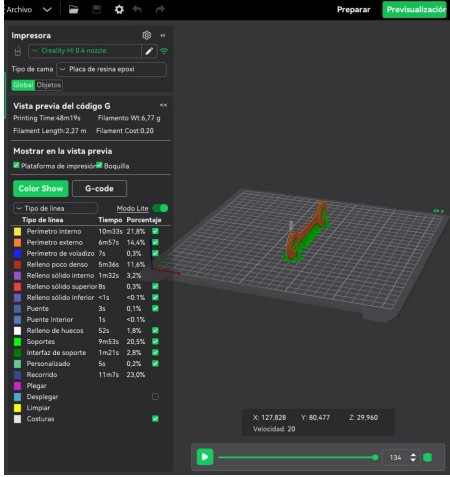
\includegraphics[width=\linewidth]{anexo/lam_a.jpg}\caption{}\end{subfigure}\hfill
\begin{subfigure}[t]{0.38\textwidth}\centering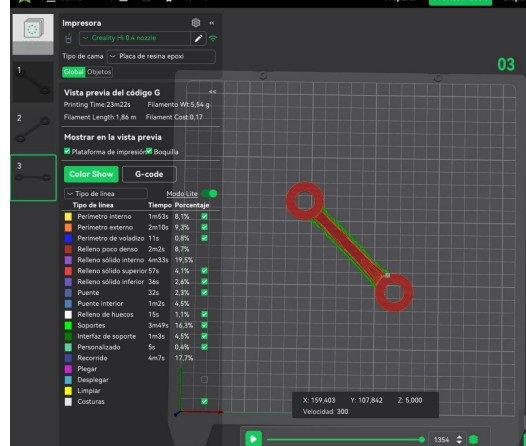
\includegraphics[width=\linewidth]{anexo/lam_b.jpg}\caption{}\end{subfigure}
\caption{Vista previa del código G en Creality Print para las orientaciones vertical y horizontal.}\label{fig:tiempo}
\par\footnotesize\textit{Nota.} Captura de pantalla de Creality Print (impresora Creality Hi 0.4 nozzle). Se muestran el tiempo de impresión, la masa y la longitud de filamento y el reparto del tiempo por tipo de línea.
\end{figure*}
\begin{table*}[t]
\caption{Resumen de resultados por condición (media de G1 y G2)}\label{tab:resultados}
\centering\small
\begin{tabular}{@{}llccccccc@{}}\toprule
 & & \multicolumn{3}{c}{Fuerza máxima (N)} & \multicolumn{3}{c}{Deformación (mm)} & Masa \\
\cmidrule(lr){3-5}\cmidrule(lr){6-8}
Configuración & Orient. & Tensión & Compresión & Flexión & Tensión & Compresión & Flexión & (g) \\\midrule
Fina & 90° & 69{,}8 & 141{,}2 & 32{,}2 & 1{,}2 & 3{,}0 & 4{,}3 & 4{,}2 \\
 & 45° & 91{,}2 & 158{,}6 & 47{,}5 & 2{,}2 & 3{,}3 & 6{,}9 & 4{,}3 \\
 & 0° & 115{,}6 & 175{,}3 & 60{,}2 & 2{,}8 & 3{,}7 & 8{,}8 & 4{,}4 \\
\midrule
Estándar & 90° & 75{,}9 & 156{,}1 & 35{,}6 & 1{,}4 & 3{,}4 & 4{,}8 & 5{,}3 \\
 & 45° & 104{,}3 & 174{,}9 & 53{,}5 & 2{,}6 & 3{,}8 & 7{,}7 & 5{,}4 \\
 & 0° & 131{,}3 & 193{,}8 & 67{,}8 & 3{,}2 & 4{,}1 & 9{,}6 & 5{,}5 \\
\midrule
Fuerte & 90° & 106{,}9 & 238{,}6 & 58{,}3 & 2{,}1 & 5{,}6 & 7{,}9 & 8{,}9 \\
 & 45° & 155{,}2 & 268{,}0 & 80{,}2 & 3{,}9 & 6{,}2 & 11{,}8 & 9{,}1 \\
 & 0° & 190{,}6 & 295{,}0 & 98{,}8 & 4{,}7 & 6{,}8 & 14{,}5 & 9{,}2 \\
\bottomrule
\end{tabular}
\\[2pt]
\footnotesize\textit{Nota.} Elaboración propia. Medias de las geometrías G1 y G2 (una probeta por geometría y condición). Orient.: ángulo del eje de la pieza respecto de la cama. Masa: media de los tres ensayos. Datos completos en \texttt{datos/resultados.csv}.
\end{table*}
\begin{figure*}[t]
\centering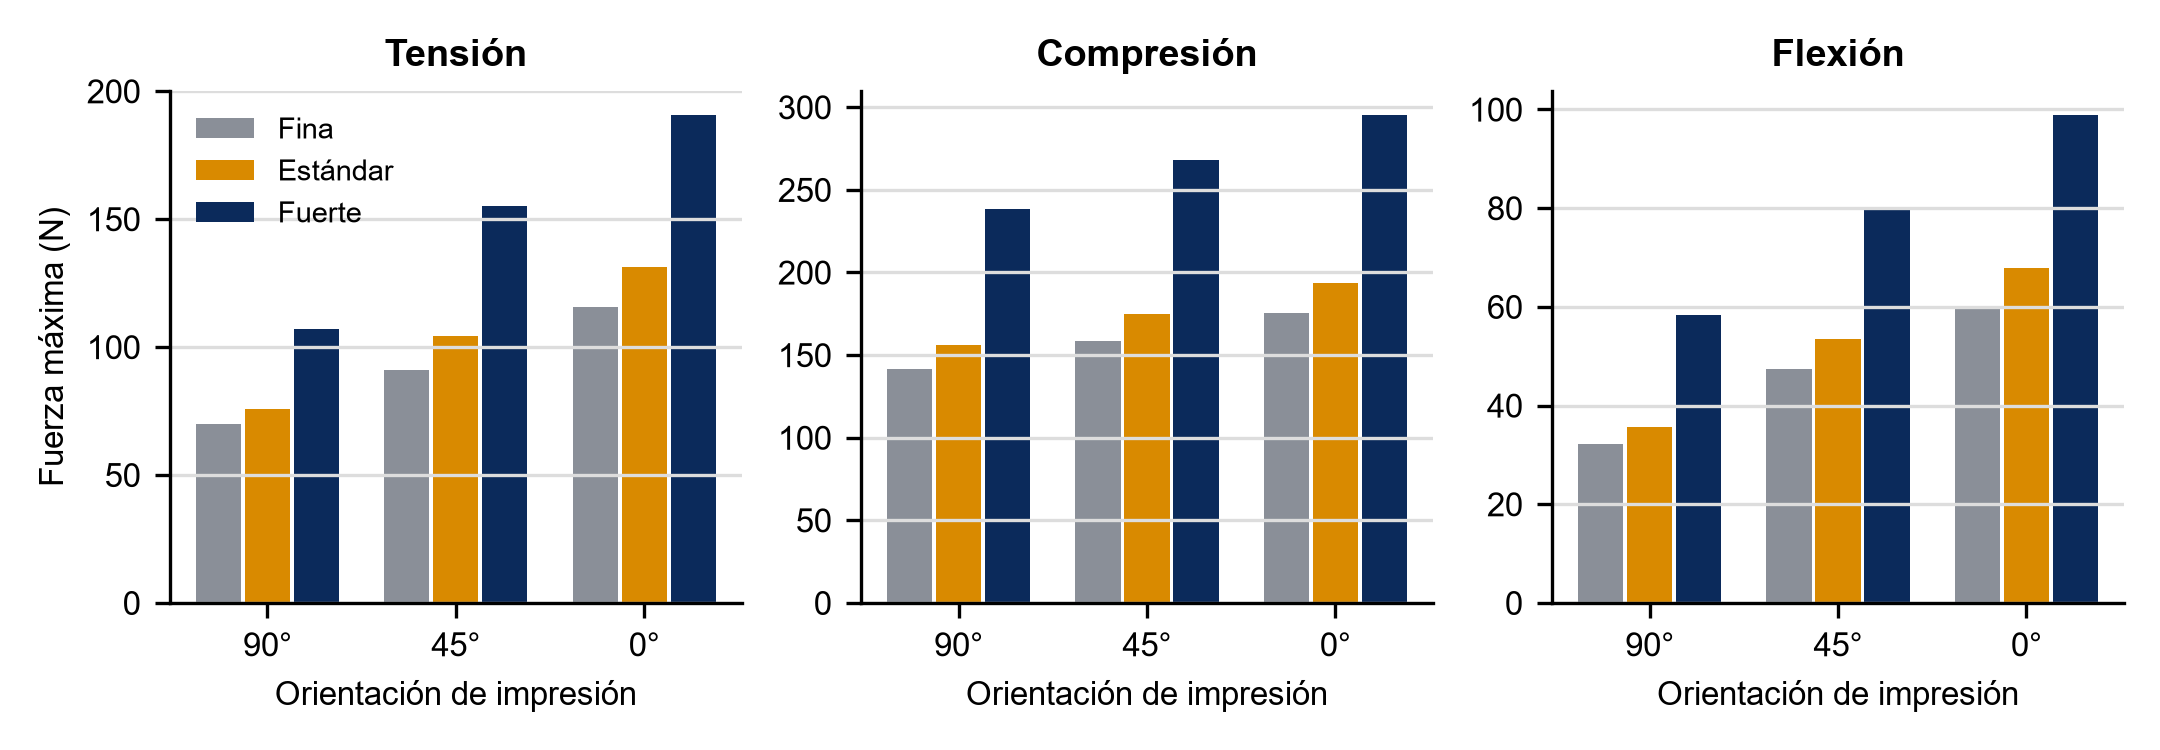
\includegraphics[width=0.85\textwidth]{../figuras/fig5_resultados_articulo.png}
\caption{Fuerza máxima por configuración y orientación en cada ensayo.}\label{fig:resultados}
\par\footnotesize\textit{Nota.} Elaboración propia. Barras: media de G1 y G2.
\end{figure*}
\begin{figure}[t]
\centering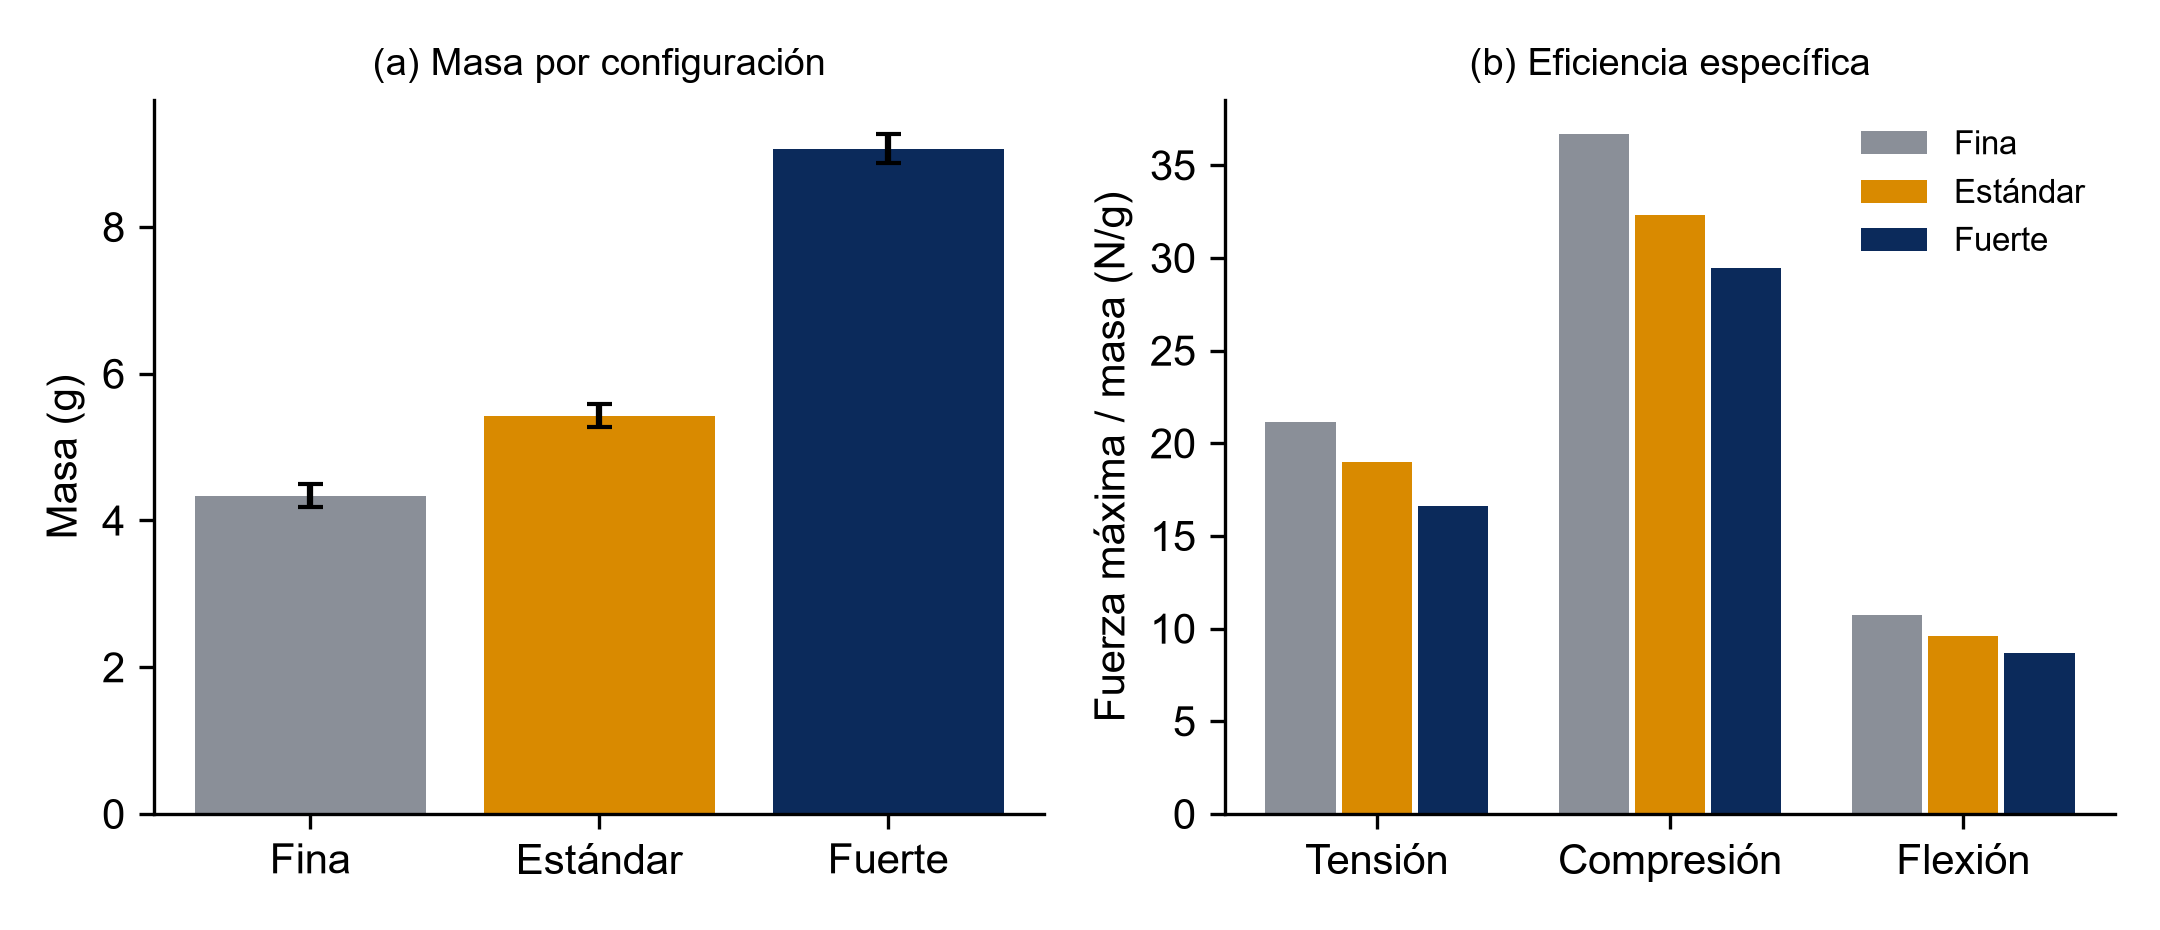
\includegraphics[width=\columnwidth]{../figuras/fig2_eficiencia.png}
\caption{Masa y fuerza máxima por gramo según la configuración.}\label{fig:eficiencia}
\par\footnotesize\textit{Nota.} Elaboración propia. (a) Media $\pm$ desviación de las 18 probetas de cada configuración. (b) Media de la razón $F/m$ de 6 probetas por barra.
\end{figure}
\begin{figure}[t]
\centering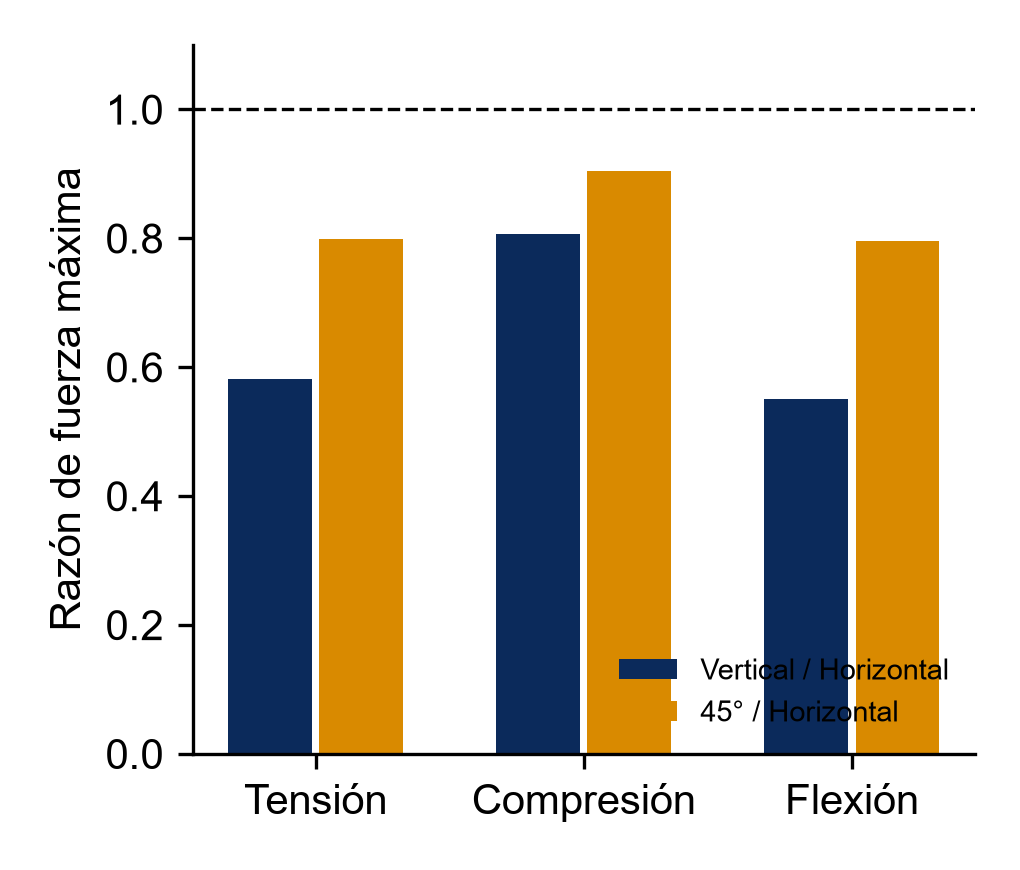
\includegraphics[width=0.7\columnwidth]{../figuras/fig3_anisotropia.png}
\caption{Razón de fuerza máxima respecto de la orientación horizontal.}\label{fig:aniso}
\par\footnotesize\textit{Nota.} Elaboración propia. Razón = fuerza en la orientación indicada / fuerza en 0°, promedio de configuraciones y geometrías.
\end{figure}
% ---------------- V. DISCUSION ----------------
\section{Discusión}
Los resultados registrados permiten comparar el efecto conjunto de las configuraciones de impresión, la orientación de fabricación y la geometría generativa sobre el comportamiento mecánico de piezas fabricadas en PLA. En los tres tipos de ensayo, la configuración Fuerte presentó las mayores fuerzas máximas, mientras que la orientación horizontal mostró consistentemente un mejor desempeño en términos de capacidad de carga. Sin embargo, el aumento de fuerza estuvo acompañado de un incremento considerable en la cantidad de material utilizado. La evaluación conjunta de fuerza máxima, deformación y masa permitió identificar diferencias entre el desempeño absoluto y la eficiencia relativa de las configuraciones estudiadas.

La influencia de la orientación de fabricación sobre la fuerza máxima registrada resulta coherente con el comportamiento anisotrópico descrito en la literatura sobre impresión FDM. Chacón et al. (2017) identificaron diferencias relevantes en el comportamiento mecánico de piezas de PLA según la orientación y otros parámetros de fabricación. En el presente estudio, las probetas horizontales registraron las mayores fuerzas máximas, mientras que las orientaciones verticales presentaron valores inferiores y modos de falla asociados a las interfaces entre capas, especialmente en tensión y flexión. Este comportamiento puede relacionarse con la disposición de los cordones depositados respecto a la dirección de carga y con la resistencia de sus uniones. No obstante, las diferencias observadas también pueden verse influenciadas por la geometría particular de cada probeta, la trayectoria de deposición y las condiciones de aplicación manual de carga.

La comparación de las configuraciones de impresión evidencia que una mayor fuerza máxima no implica necesariamente una mayor eficiencia por unidad de masa. Aunque la configuración Fuerte soportó las mayores cargas en los tres ensayos, también presentó el mayor consumo de material, reduciendo su relación fuerza/masa frente a la configuración Fina. Este resultado adquiere importancia en aplicaciones donde la reducción de peso constituye un criterio relevante de diseño. Sin embargo, no debe interpretarse como una superioridad general de la configuración Fina, debido a que la selección de parámetros depende de las condiciones de carga y de los requisitos funcionales de cada componente. Además, las configuraciones evaluadas modificaron simultáneamente diferentes parámetros, por lo que no es posible determinar de manera independiente cuánto contribuyeron las paredes, el porcentaje de relleno o el patrón interno a los cambios registrados.

La interpretación de los resultados debe considerar varias limitaciones metodológicas. En primer lugar, se utilizó una sola probeta por combinación experimental, lo que impide estimar adecuadamente la repetibilidad de las mediciones y la variabilidad propia del proceso de fabricación. En segundo lugar, los ensayos fueron realizados mediante aplicación manual de carga, sin un control normalizado de velocidad ni un registro completo de curvas fuerza-desplazamiento. Adicionalmente, el estudio empleó un único material PLA y configuraciones de impresión que agrupan varios parámetros, impidiendo aislar sus efectos individuales. Tampoco se documentó un procedimiento de acondicionamiento previo de las probetas ni una caracterización completa de sus dimensiones y secciones resistentes. En consecuencia, los resultados deben interpretarse como tendencias exploratorias de fuerza máxima y deformación, y no como una caracterización normalizada de propiedades mecánicas intrínsecas del material.

Entre las principales fortalezas del estudio se encuentra la comparación sistemática de dos alternativas geométricas generativas para cada tipo de ensayo, fabricadas bajo condiciones equivalentes de impresión. Asimismo, la incorporación de tres orientaciones y tres configuraciones permite examinar diferencias de comportamiento entre piezas sometidas a tensión, compresión y flexión. La inclusión de la masa y de la relación fuerza/masa amplía el análisis más allá de la capacidad absoluta de carga y permite explorar criterios de eficiencia estructural. Finalmente, el estudio integra herramientas de diseño computacional, laminado, fabricación aditiva y evaluación mecánica en un mismo procedimiento, proporcionando una base metodológica para investigaciones posteriores de mayor alcance experimental.
% ---------------- VI. CONCLUSIONES ----------------
\section{Conclusiones}
La investigación permitió analizar comparativamente la influencia de la orientación de fabricación, las configuraciones FDM y las geometrías generativas sobre la fuerza máxima, la deformación y la masa de piezas de PLA sometidas a tensión, compresión y flexión. Los resultados registrados indicaron que la orientación horizontal presentó las mayores capacidades de carga en las condiciones evaluadas, mientras que la configuración Fuerte alcanzó los valores máximos de fuerza en los tres ensayos. Sin embargo, el mayor consumo de material asociado a esta configuración redujo su desempeño relativo cuando se consideró la relación fuerza/masa. Las diferencias entre las geometrías G1 y G2 fueron menores que las observadas entre configuraciones y orientaciones, aunque se requiere replicación experimental para determinar su significancia.

El principal aporte del estudio consiste en mostrar la importancia de considerar conjuntamente la capacidad de carga y la eficiencia material al seleccionar configuraciones de impresión para piezas diseñadas generativamente. En aplicaciones donde la fuerza máxima constituye el criterio principal, las configuraciones reforzadas pueden resultar favorables, mientras que en componentes con restricciones de masa conviene evaluar alternativas con menor consumo de filamento. Por ello, se recomienda incorporar la orientación de fabricación desde las etapas iniciales de diseño y comparar diferentes configuraciones mediante indicadores que relacionen el desempeño estructural con la cantidad de material utilizado. Estas decisiones deben validarse experimentalmente según las condiciones de servicio previstas.

Como continuación de esta investigación se propone desarrollar un diseño experimental que permita modificar independientemente la densidad de relleno, el número de paredes, la altura de capa, el patrón interno y la orientación de fabricación, incorporando varias réplicas por condición. Asimismo, se recomienda utilizar una máquina universal de ensayos para obtener curvas fuerza-desplazamiento y determinar propiedades mecánicas normalizadas mediante probetas apropiadas. Otra línea de investigación consiste en comparar geometrías generativas con modelos convencionales de referencia, evaluando simultáneamente masa, rigidez, capacidad de carga y tiempo de fabricación. Finalmente, sería relevante ampliar el análisis hacia materiales como PETG y TPU, con el propósito de estudiar diferencias en flexibilidad, deformación recuperable y absorción de energía.
% ---------------- VII. DECLARACIONES ----------------
\section{Declaraciones}
\subsection{Contribución de la autora (CRediT)}
A.D.N.R.: conceptualización, desarrollo metodológico, investigación, diseño y modelado tridimensional, preparación de modelos para manufactura aditiva, análisis formal de resultados, visualización de datos, redacción del manuscrito y revisión de su contenido.
\subsection{Financiación}
La presente investigación se desarrolló en el contexto académico del Seminario de Investigación de la Universidad Ean.
\subsection{Conflicto de intereses}
La autora declara no tener conflictos de intereses financieros, comerciales o personales que puedan influir en la interpretación o presentación de los resultados de esta investigación.
\subsection{Disponibilidad de datos}
Los resultados experimentales utilizados en este estudio se encuentran organizados en el archivo \texttt{resultados.csv}, que contiene las mediciones correspondientes a las combinaciones de geometría, configuración de impresión, orientación y tipo de ensayo. Están disponibles, junto con las figuras y los programas de análisis, en \url{https://github.com/IngDinoAlip/impresion3d-fdm-pla}.
\subsection{Uso de inteligencia artificial}
Durante la preparación del manuscrito se utilizaron herramientas de inteligencia artificial como apoyo para la organización, revisión lingüística y mejora de la redacción académica. La autora conserva la responsabilidad sobre el contenido científico, la veracidad de los datos experimentales, la revisión de las fuentes y las conclusiones presentadas.
% ---------------- VIII. REFERENCIAS ----------------
\section{Referencias}
{\footnotesize\setlength{\parindent}{-1.2em}\setlength{\leftskip}{1.2em}\raggedright
Alafaghani, A., Qattawi, A., Alrawi, B., \& Guzman, A. (2017). Experimental optimization of fused deposition modelling processing parameters: A design-for-manufacturing approach. \textit{Procedia Manufacturing}, \textit{10}, 791–803. \url{https://doi.org/10.1016/j.promfg.2017.07.079}\par
Al-Tamimi, A. A., Pandžić, A., \& Kadrić, E. (2023). Investigation and prediction of tensile, flexural, and compressive properties of tough PLA material using definitive screening design. \textit{Polymers}, \textit{15}(20), 4169. \url{https://doi.org/10.3390/polym15204169}\par
Ambati, S. S., \& Ambatipudi, R. (2022). Effect of infill density and infill pattern on the mechanical properties of 3D printed PLA parts. \textit{Materials Today: Proceedings}, \textit{64}, 804–807. \url{https://doi.org/10.1016/j.matpr.2022.05.312}\par
Araque, O., Sánchez-Echeverri, L. A., \& Cerón, I. X. (2025). Impact of printing angle and layer height on the mechanical strength of PLA reinforced with chopped carbon fibres using FDM 3D printing. \textit{Polymers}, \textit{17}(22), 3069. \url{https://doi.org/10.3390/polym17223069}\par
Autodesk. (s.~f.-a). \textit{Preserve geometry}. Autodesk Fusion Help. \url{https://help.autodesk.com/cloudhelp/ENU/Fusion-GenerativeDesign/files/GD-PRESERVE-GEOM.htm}\par
Autodesk. (s.~f.-b). \textit{Specify objectives in the Generative Design workspace}. Autodesk Fusion Help. \url{https://help.autodesk.com/view/fusion360/ENU/?contextId=GD-SPECIFY-OBJECTIVES}\par
Ben hadj Hassine, S., Chatti, S., Louhichi, B., \& Seibi, A. (2024). Experimental study of the tensile behavior of structures obtained by FDM 3D printing process. \textit{Polymers}, \textit{16}(11), 1562. \url{https://doi.org/10.3390/polym16111562}\par
Birosz, M. T., \& Andó, M. (2023). Effect of infill pattern scaling on mechanical properties of FDM-printed PLA specimens. \textit{Progress in Additive Manufacturing}, \textit{9}(4), 875–883. \url{https://doi.org/10.1007/s40964-023-00487-8}\par
Buss, C., Reci, F., Hribernig, T., \& Steininger, S. (2026). Experimental investigation into the influence of infill density, print pattern, and built-up direction on the flexural strength of FFF-manufactured PLA components. \textit{Journal of Manufacturing and Materials Processing}, \textit{10}(1), 21. \url{https://doi.org/10.3390/jmmp10010021}\par
Chacón, J. M., Caminero, M. A., García-Plaza, E., \& Núñez, P. J. (2017). Additive manufacturing of PLA structures using fused deposition modelling: Effect of process parameters on mechanical properties and their optimal selection. \textit{Materials \& Design}, \textit{124}, 143–157. \url{https://doi.org/10.1016/j.matdes.2017.03.065}\par
Chalgham, A., Ehrmann, A., \& Wickenkamp, I. (2021). Mechanical properties of FDM printed PLA parts before and after thermal treatment. \textit{Polymers}, \textit{13}(8), 1239. \url{https://doi.org/10.3390/polym13081239}\par
Cojocaru, V., Frunzaverde, D., Miclosina, C. O., \& Marginean, G. (2022). The influence of the process parameters on the mechanical properties of PLA specimens produced by fused filament fabrication—a review. \textit{Polymers}, \textit{14}(5), 886. \url{https://doi.org/10.3390/polym14050886}\par
Dziewit, P., Rajkowski, K., \& Płatek, P. (2024). Effects of building orientation and raster angle on the mechanical properties of selected materials used in FFF techniques. \textit{Materials}, \textit{17}(24), 6076. \url{https://doi.org/10.3390/ma17246076}\par
Ergüder, T. O., \& Bulut, C. (2025). Mechanical characterization of FDM-printed PLA: Role of infill geometry and build direction. \textit{Challenge Journal of Structural Mechanics}, \textit{11}(4), 201. \url{https://doi.org/10.20528/cjsmec.2025.04.003}\par
Ganeshkumar, S., Kumar, S. D., Magarajan, U., Rajkumar, S., Arulmurugan, B., Sharma, S., Li, C., Ilyas, R. A., \& Badran, M. F. (2022). Investigation of tensile properties of different infill pattern structures of 3D-printed PLA polymers: Analysis and validation using finite element analysis in ANSYS. \textit{Materials}, \textit{15}(15), 5142. \url{https://doi.org/10.3390/ma15155142}\par
Gocyk, K., Afshar, R., \& Abali, B. E. (2026). On strength variations effected by infill patterns such as honeycomb, gyroid, and Archimedean chords used in additive manufacturing. \textit{Polymers}, \textit{18}(13), 1619. \url{https://doi.org/10.3390/polym18131619}\par
Hallaert, M., Ammar, A., Kanit, T., \& Ayoub, G. (2026). Influence of infill density, pattern, and contour width on the mechanical behavior of 3D-printed PLA components. \textit{Results in Materials}, \textit{31}, 100987. \url{https://doi.org/10.1016/j.rinma.2026.100987}\par
Kadhum, A. H., Al-Zubaidi, S., \& Abdulkareem, S. S. (2023). Effect of the infill patterns on the mechanical and surface characteristics of 3D printing of PLA, PLA+ and PETG materials. \textit{ChemEngineering}, \textit{7}(3), 46. \url{https://doi.org/10.3390/chemengineering7030046}\par
Khaliq, J., Gurrapu, D. R., \& Elfakhri, F. (2023). Effects of infill line multiplier and patterns on mechanical properties of lightweight and resilient hollow section products manufactured using fused filament fabrication. \textit{Polymers}, \textit{15}(12), 2585. \url{https://doi.org/10.3390/polym15122585}\par
Medibew, T. M. (2022). A comprehensive review on the optimization of the fused deposition modeling process parameter for better tensile strength of PLA-printed parts. \textit{Advances in Materials Science and Engineering}, \textit{2022}, 1–11. \url{https://doi.org/10.1155/2022/5490831}\par
Mencarelli, M., Sisella, M., Puggelli, L., Innocenti, B., \& Volpe, Y. (2025). Sensitivity analysis of 3D printing parameters on mechanical properties of fused deposition modeling-printed polylactic acid parts. \textit{Applied Mechanics}, \textit{6}(1), 17. \url{https://doi.org/10.3390/applmech6010017}\par
Mohan, E., \& Saravana Kumar, M. (2022). Experimental investigation on mechanical and tribological properties of the fused filament fabrication of poly-lactic acid parts with various print orientations. \textit{Applied Physics A}, \textit{128}(5), 428. \url{https://doi.org/10.1007/s00339-022-05579-w}\par
Pernet, B., Nagel, J. K., \& Zhang, H. (2022). Compressive strength assessment of 3D printing infill patterns. \textit{Procedia CIRP}, \textit{105}, 682–687. \url{https://doi.org/10.1016/j.procir.2022.02.114}\par
Srivastava, J., \& Kawakami, H. (2023). Systematic review of difference between topology optimization and generative design. \textit{IFAC-PapersOnLine}, \textit{56}(2), 6561–6568. \url{https://doi.org/10.1016/j.ifacol.2023.10.307}\par
Tattimbetova, G., Kapustynskyi, O., Rakishev, A., Škamat, J., \& Zhetessova, G. (2026). Effect of infill pattern, density, and orientation on the mechanical and surface characteristics of MEX-printed PLA samples for casting-pattern applications. \textit{Applied Sciences}, \textit{16}(17), 8538. \url{https://doi.org/10.3390/app16178538}\par
Travieso-Rodriguez, J. A., Jerez-Mesa, R., Llumà, J., Traver-Ramos, O., Gomez-Gras, G., \& Roa Rovira, J. J. (2019). Mechanical properties of 3D-printing polylactic acid parts subjected to bending stress and fatigue testing. \textit{Materials}, \textit{12}(23), 3859. \url{https://doi.org/10.3390/ma12233859}\par
Tymrak, B. M., Kreiger, M., \& Pearce, J. M. (2014). Mechanical properties of components fabricated with open-source 3-D printers under realistic environmental conditions. \textit{Materials \& Design}, \textit{58}, 242–246. \url{https://doi.org/10.1016/j.matdes.2014.02.038}\par
Vanaei, S., Rastak, M., El Magri, A., Vanaei, H. R., Raissi, K., \& Tcharkhtchi, A. (2023). Orientation-dependent mechanical behavior of 3D printed polylactic acid parts: An experimental–numerical study. \textit{Machines}, \textit{11}(12), 1086. \url{https://doi.org/10.3390/machines11121086}\par
Yan, J., Yuan, Z., Liu, Q., Liu, G., \& Li, L. (2023). Printing ready topology optimization for material extrusion polymer additive manufacturing. \textit{3D Printing and Additive Manufacturing}, \textit{10}(2), 197–212. \url{https://doi.org/10.1089/3dp.2021.0189}\par
Zhu, J., Zhou, H., Wang, C., Zhou, L., Yuan, S., \& Zhang, W. (2021). A review of topology optimization for additive manufacturing: Status and challenges. \textit{Chinese Journal of Aeronautics}, \textit{34}(1), 91–110. \url{https://doi.org/10.1016/j.cja.2020.09.020}\par
}
% ---------------- APENDICE A ----------------
\clearpage
\onecolumn
\section*{Apéndice A. Evidencia gráfica del proceso experimental}
\pendiente{Mencionar en el texto}{Citar el Apéndice A en III.3 y III.4 (p.~ej. «véanse las Figuras A1 a A7») y precisar en qué consisten los «puntos de tensión» definidos en Fusion 360 (¿carga, apoyo o ambos?).}
\begingroup\setcounter{figure}{0}\renewcommand{\thefigure}{A\arabic{figure}}
\begin{figure}[!htbp]\centering
\begin{subfigure}[t]{0.48\textwidth}\centering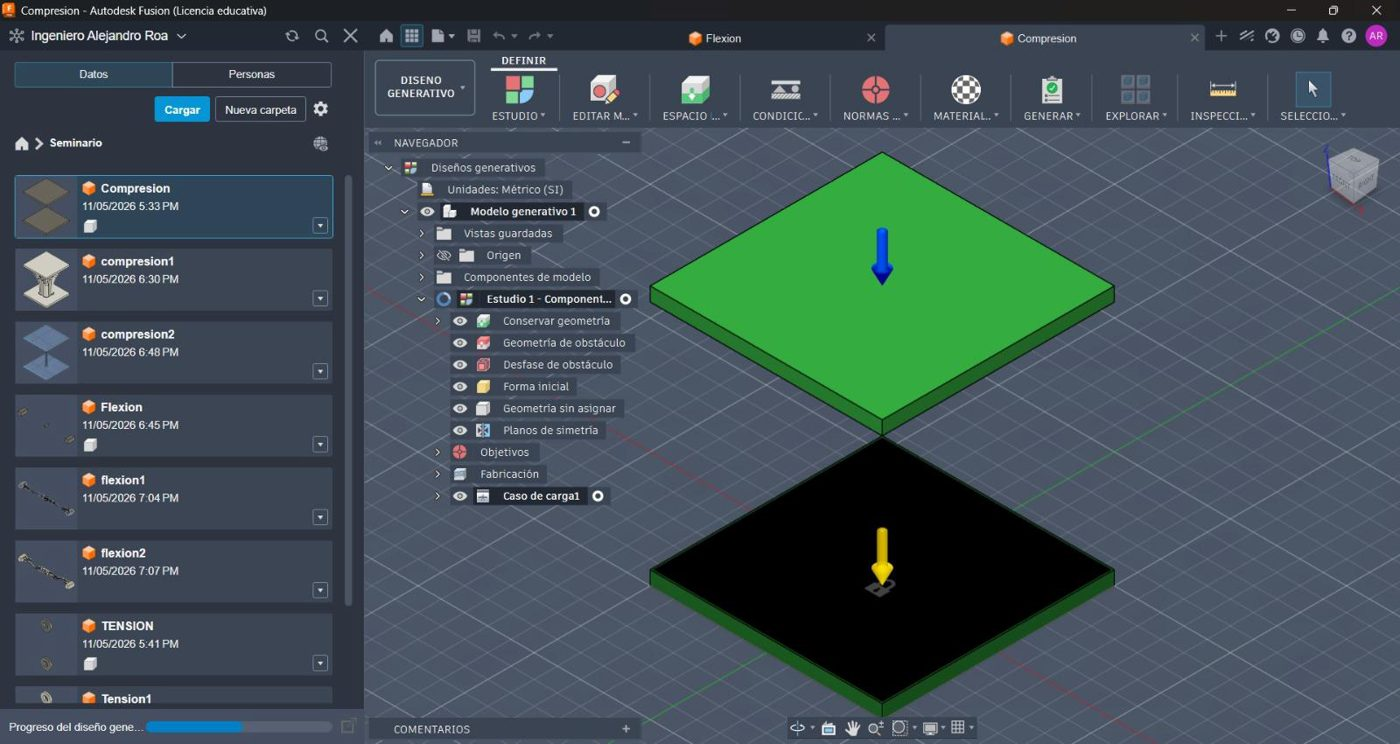
\includegraphics[width=\linewidth,height=0.20\textheight,keepaspectratio]{anexo/p13_0.jpg}\end{subfigure}\hfill
\begin{subfigure}[t]{0.48\textwidth}\centering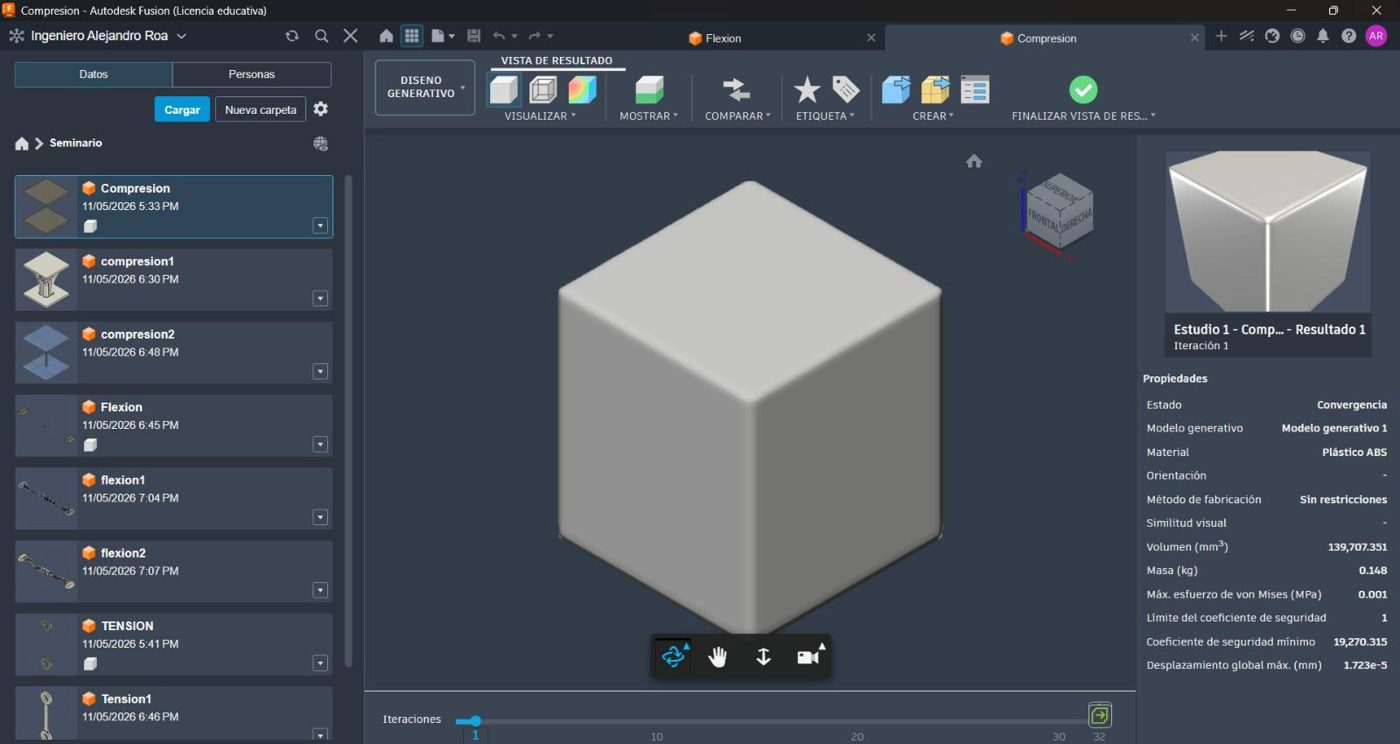
\includegraphics[width=\linewidth,height=0.20\textheight,keepaspectratio]{anexo/p13_1.jpg}\end{subfigure}\par\smallskip
\begin{subfigure}[t]{0.48\textwidth}\centering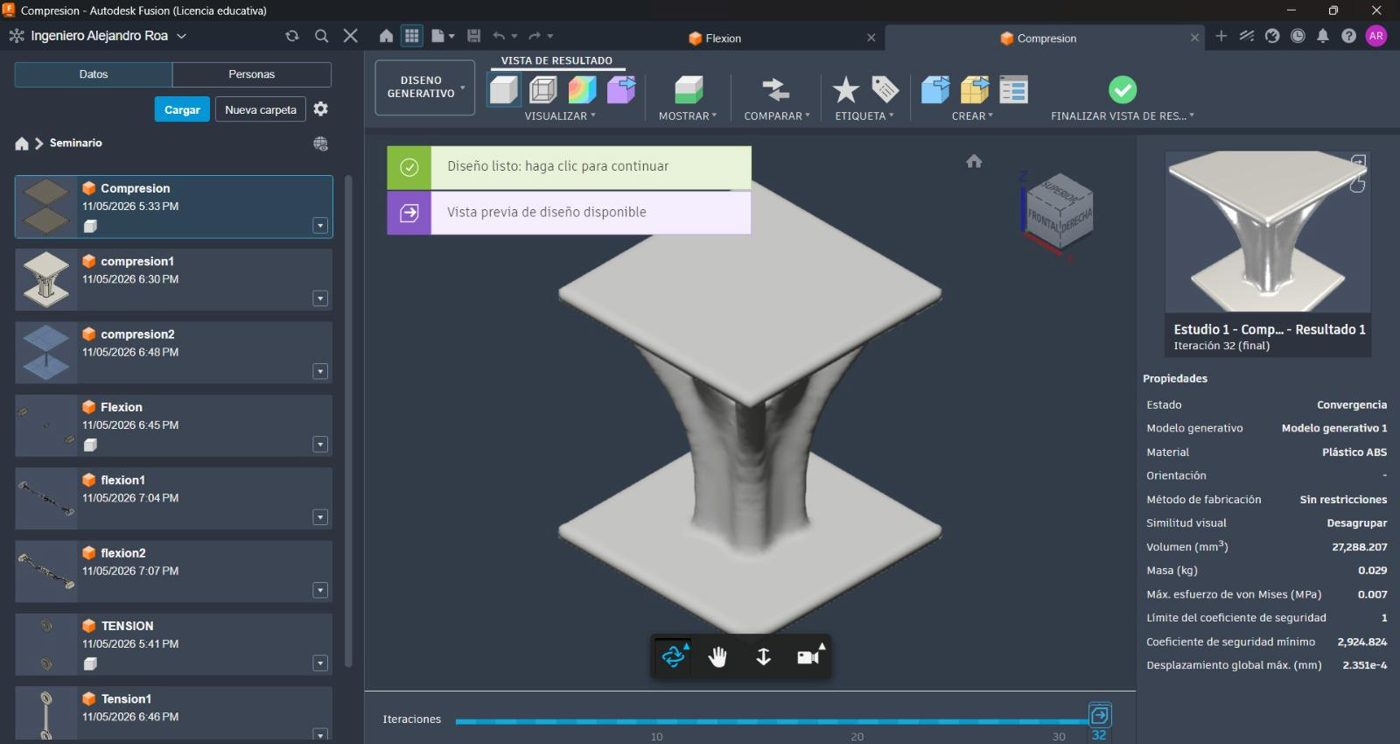
\includegraphics[width=\linewidth,height=0.20\textheight,keepaspectratio]{anexo/p14_0.jpg}\end{subfigure}\hfill
\begin{subfigure}[t]{0.48\textwidth}\centering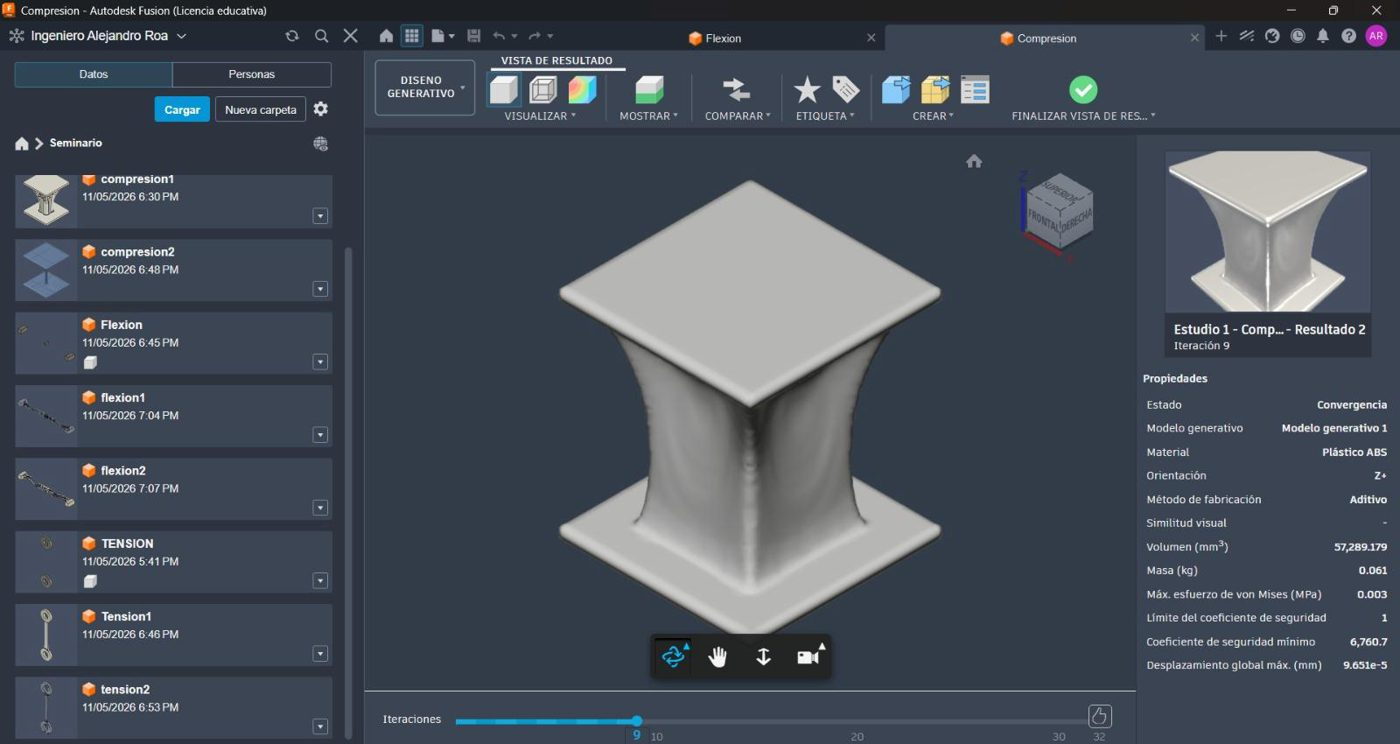
\includegraphics[width=\linewidth,height=0.20\textheight,keepaspectratio]{anexo/p14_1.jpg}\end{subfigure}\par\smallskip
\begin{subfigure}[t]{0.48\textwidth}\centering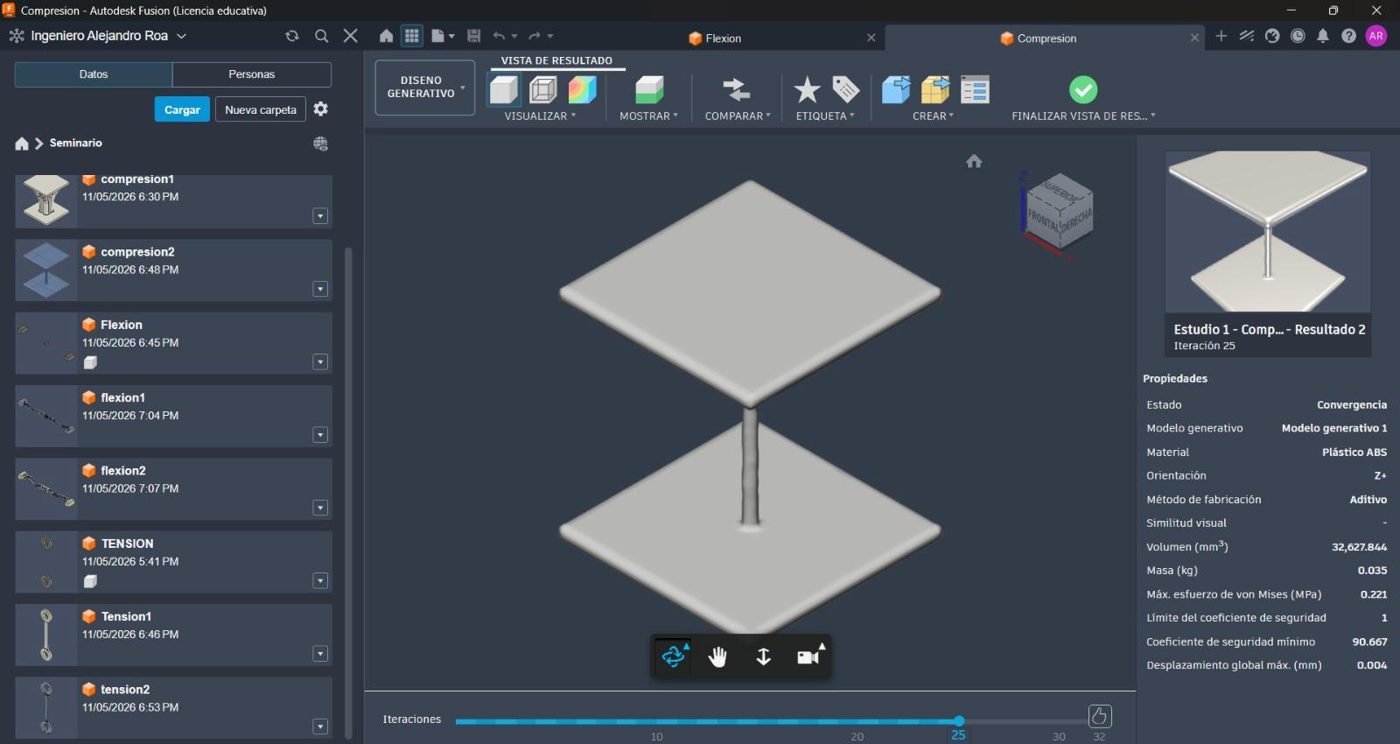
\includegraphics[width=\linewidth,height=0.20\textheight,keepaspectratio]{anexo/p15_0.jpg}\end{subfigure}\hfill
\begin{subfigure}[t]{0.48\textwidth}\centering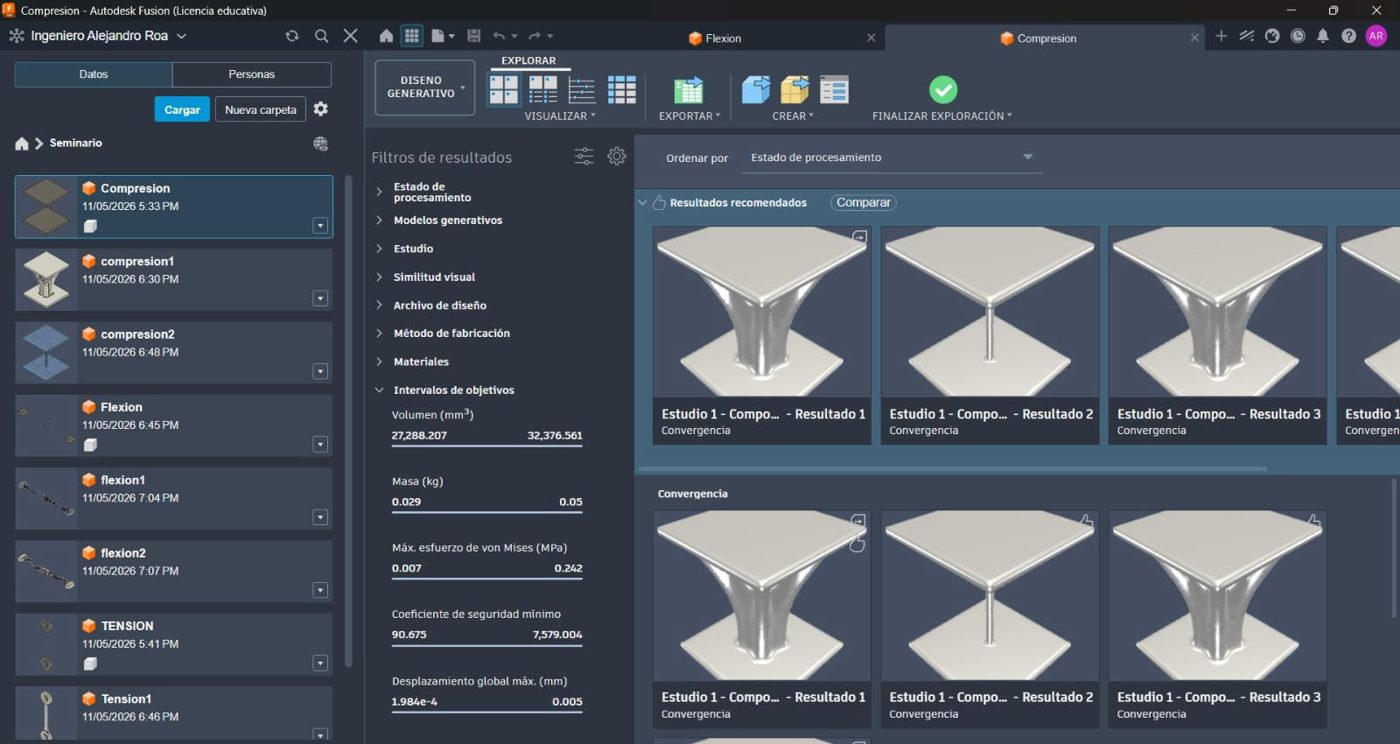
\includegraphics[width=\linewidth,height=0.20\textheight,keepaspectratio]{anexo/p15_1.jpg}\end{subfigure}\par\smallskip
\caption{Diseño generativo de la pieza de compresión en Fusion 360: definición de geometrías y cargas, espacio de diseño inicial, alternativas generadas y comparación de resultados.}
\par\footnotesize\textit{Nota.} Elaboración propia. Documento original, páginas 13 a 15.
\end{figure}
\begin{figure}[!htbp]\centering
\begin{subfigure}[t]{0.48\textwidth}\centering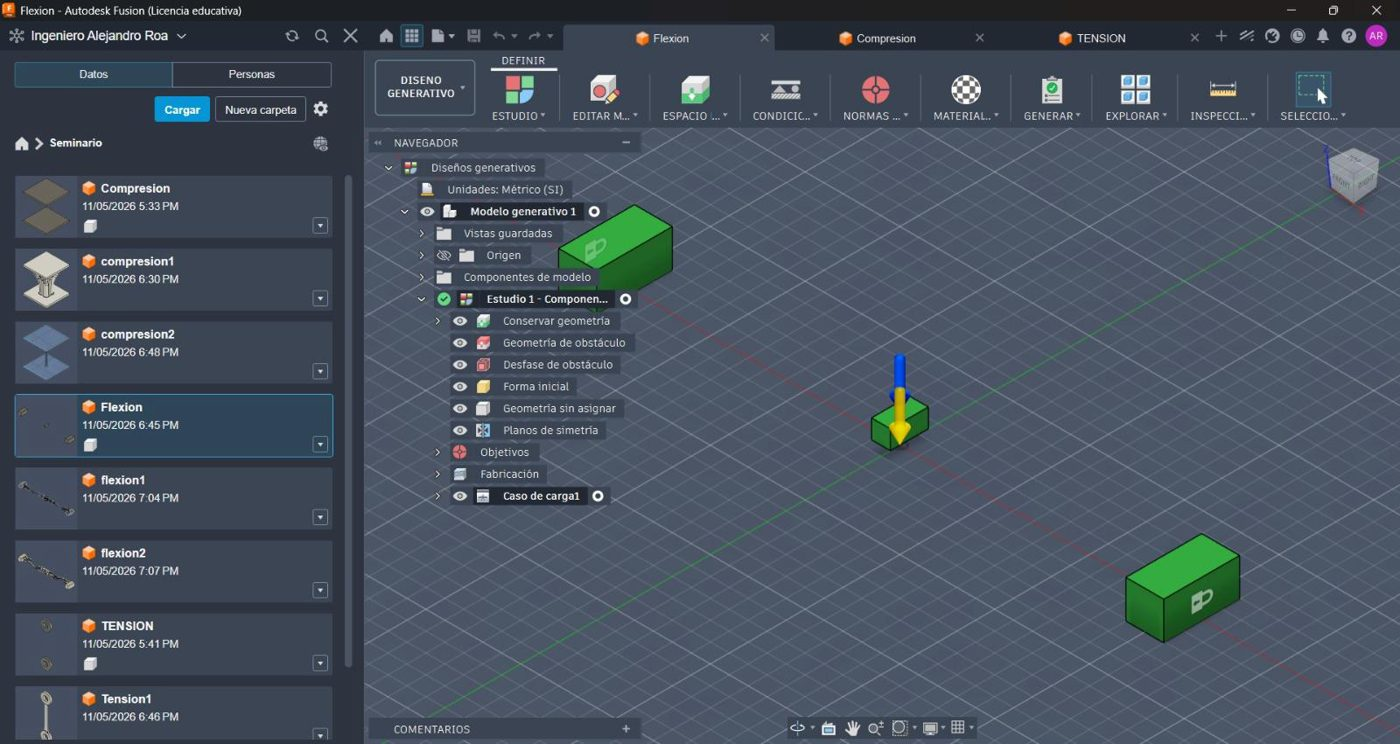
\includegraphics[width=\linewidth,height=0.20\textheight,keepaspectratio]{anexo/p18_1.jpg}\end{subfigure}\hfill
\begin{subfigure}[t]{0.48\textwidth}\centering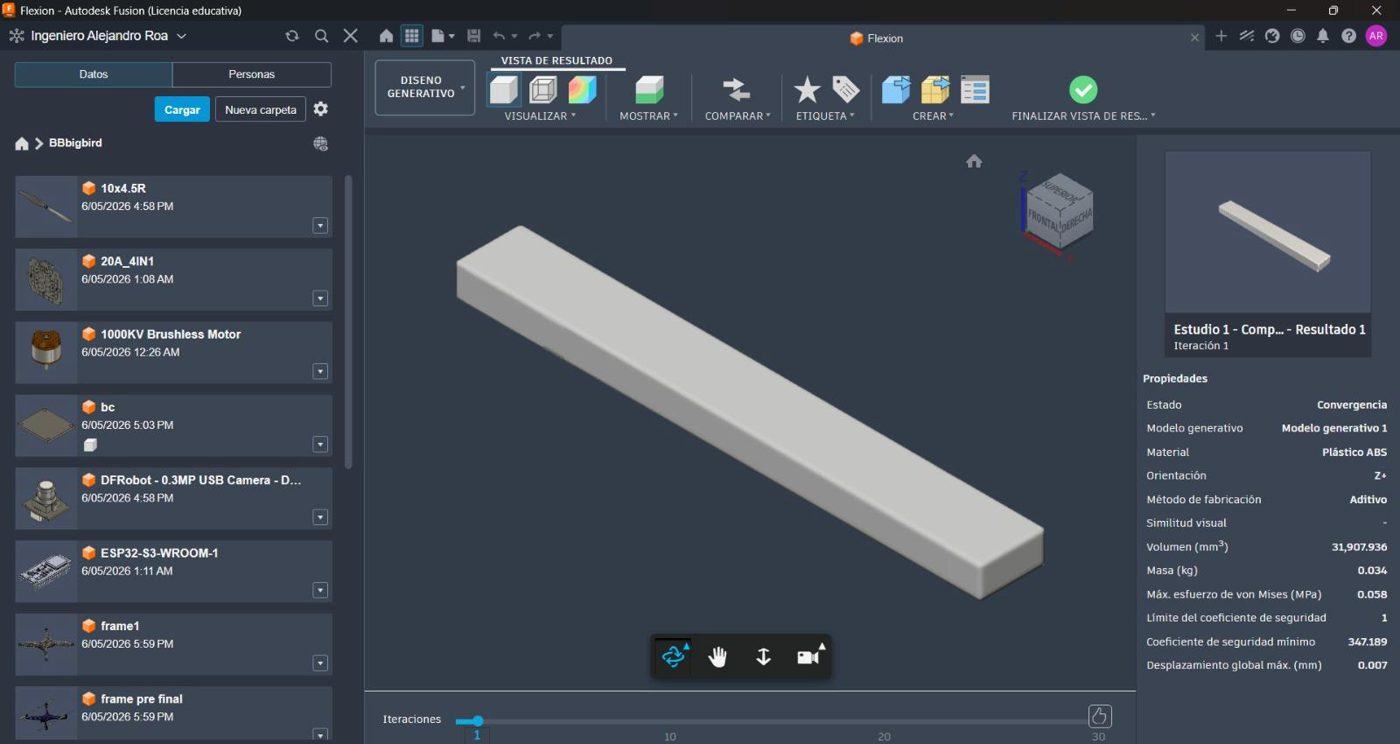
\includegraphics[width=\linewidth,height=0.20\textheight,keepaspectratio]{anexo/p16_0.jpg}\end{subfigure}\par\smallskip
\begin{subfigure}[t]{0.48\textwidth}\centering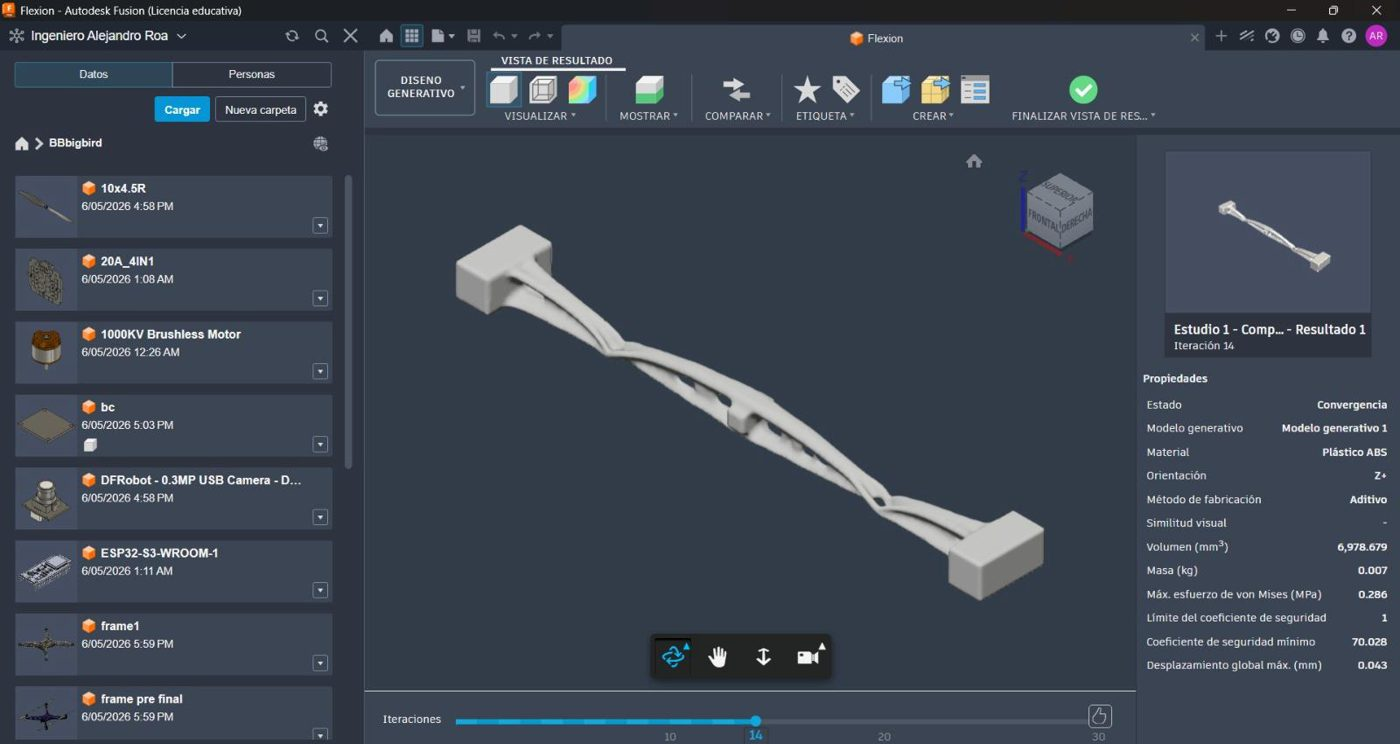
\includegraphics[width=\linewidth,height=0.20\textheight,keepaspectratio]{anexo/p16_1.jpg}\end{subfigure}\hfill
\begin{subfigure}[t]{0.48\textwidth}\centering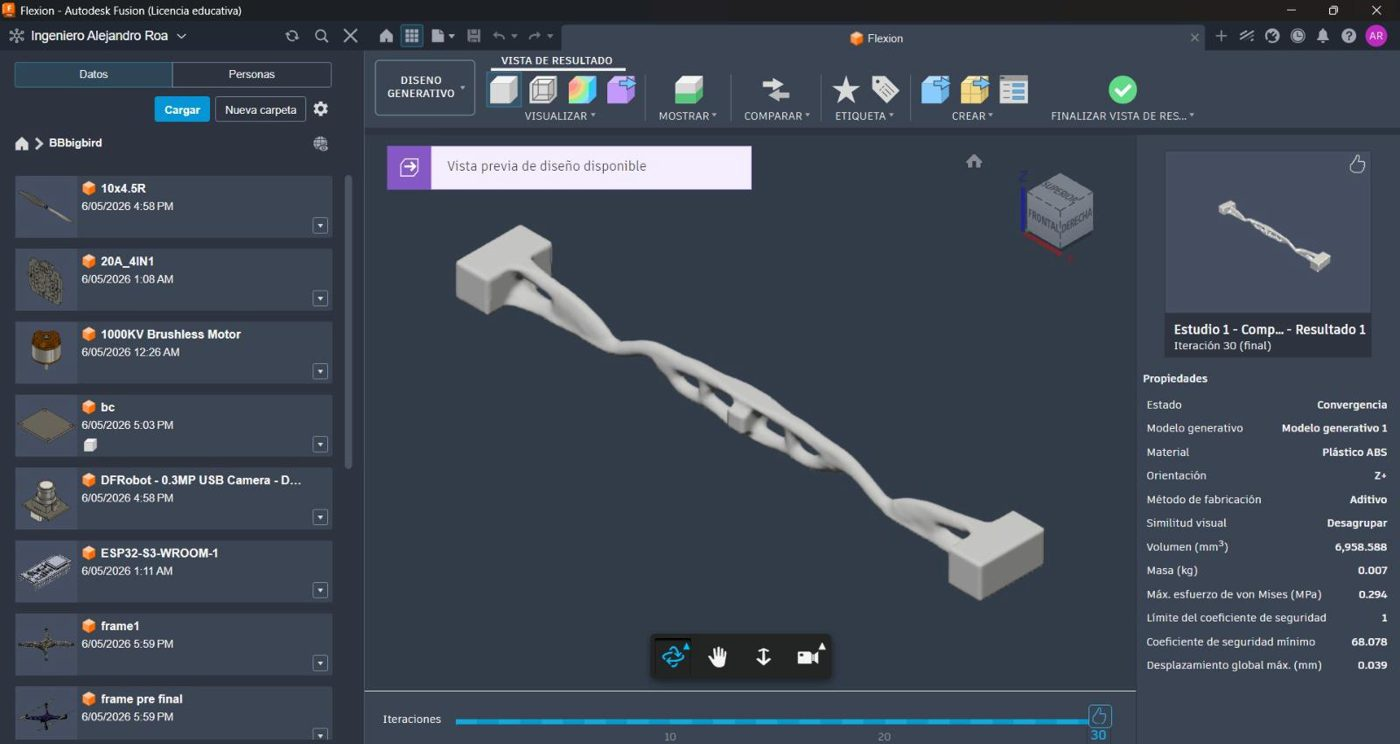
\includegraphics[width=\linewidth,height=0.20\textheight,keepaspectratio]{anexo/p17_0.jpg}\end{subfigure}\par\smallskip
\begin{subfigure}[t]{0.48\textwidth}\centering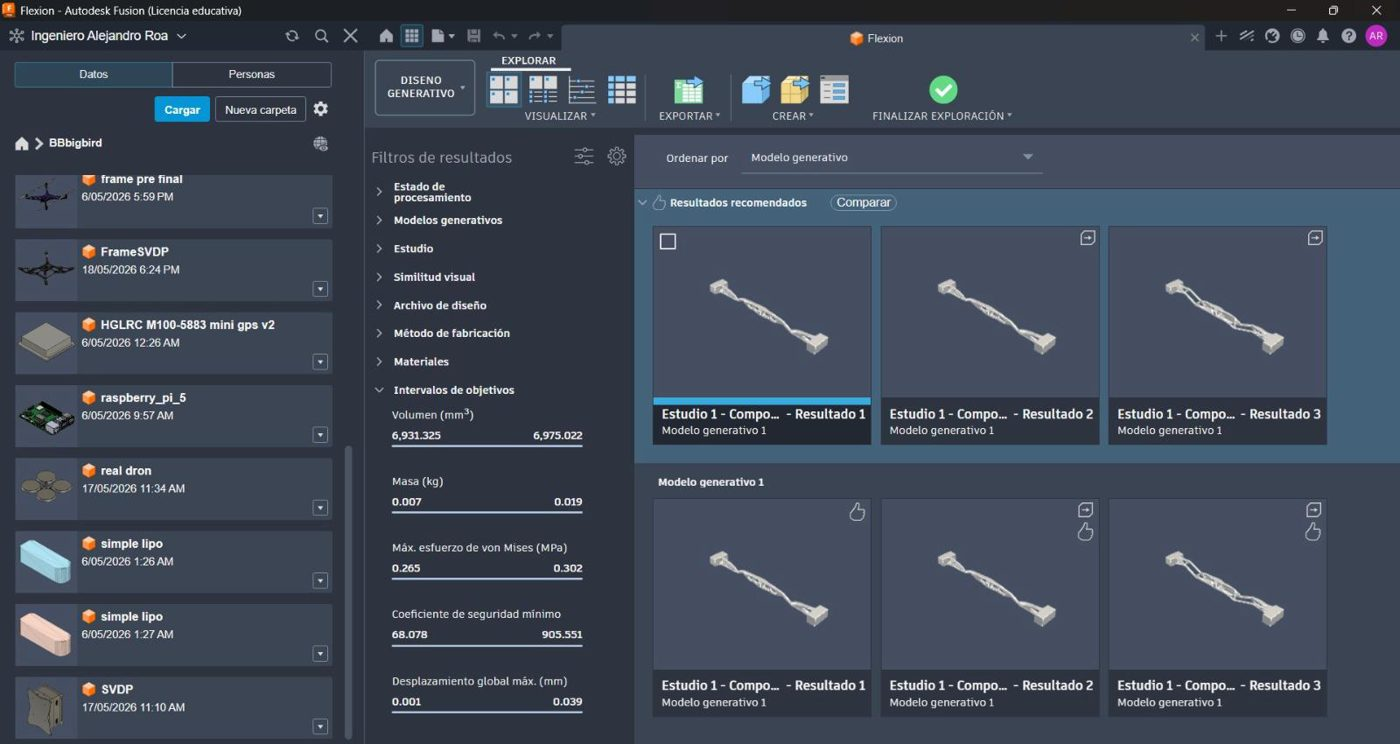
\includegraphics[width=\linewidth,height=0.20\textheight,keepaspectratio]{anexo/p17_1.jpg}\end{subfigure}\hfill
\caption{Diseño generativo de la pieza de flexión en Fusion 360: definición de geometrías y cargas, forma inicial y alternativas generadas.}
\par\footnotesize\textit{Nota.} Elaboración propia. Documento original, páginas 16 a 18.
\end{figure}
\begin{figure}[!htbp]\centering
\begin{subfigure}[t]{0.48\textwidth}\centering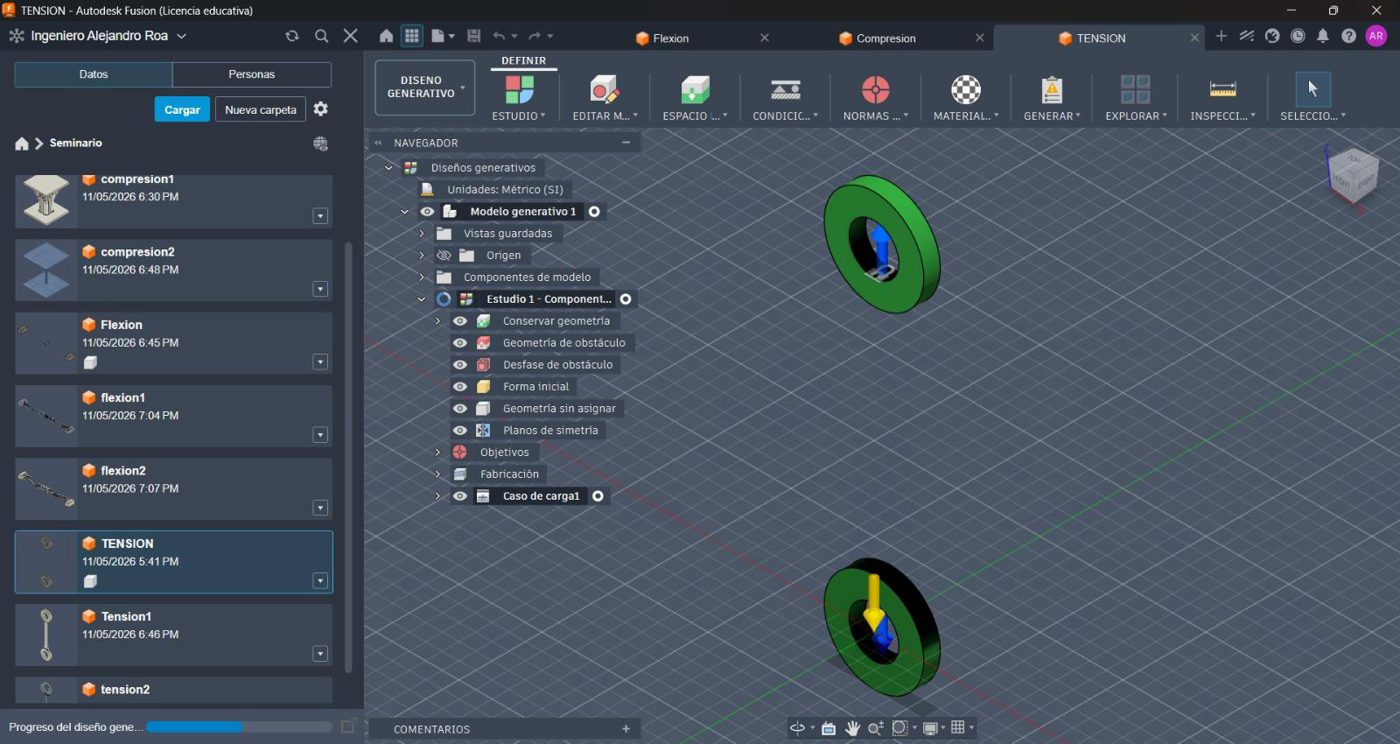
\includegraphics[width=\linewidth,height=0.20\textheight,keepaspectratio]{anexo/p18_0.jpg}\end{subfigure}\hfill
\begin{subfigure}[t]{0.48\textwidth}\centering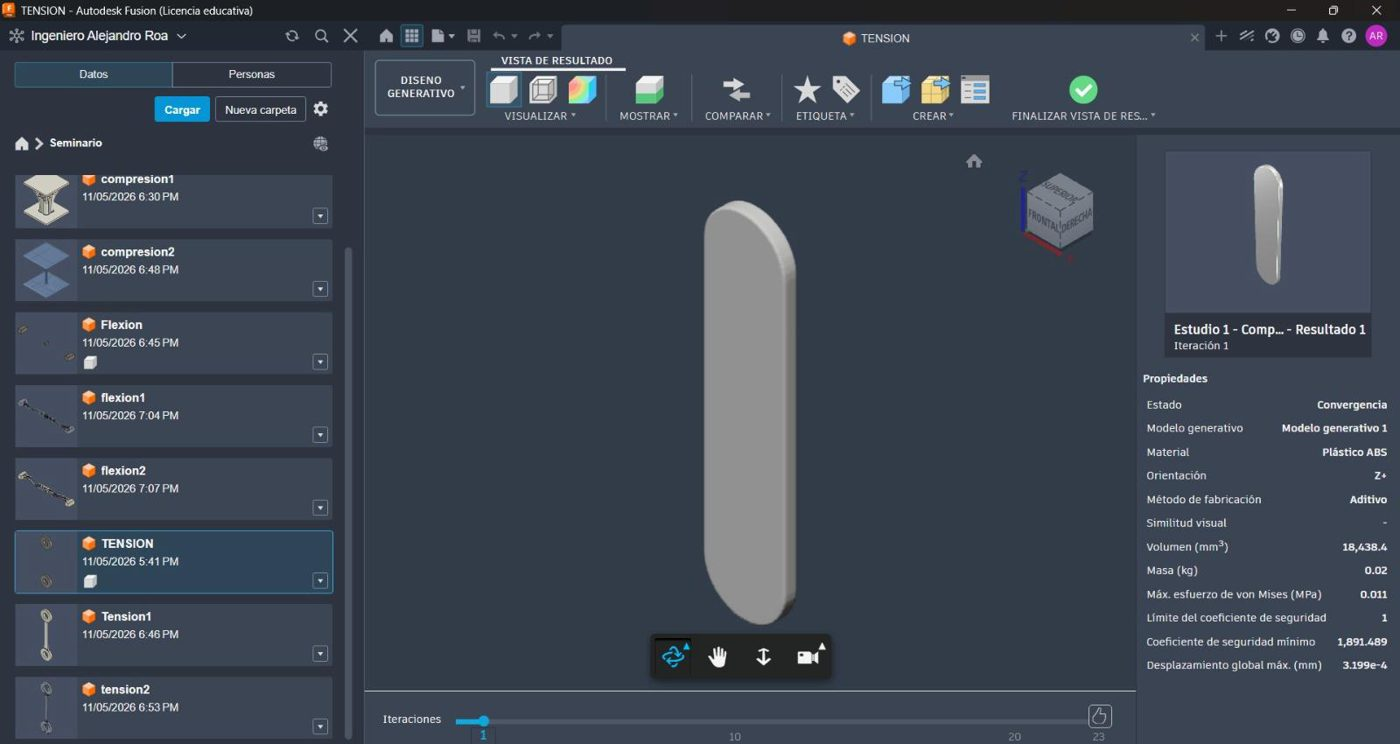
\includegraphics[width=\linewidth,height=0.20\textheight,keepaspectratio]{anexo/p19_0.jpg}\end{subfigure}\par\smallskip
\begin{subfigure}[t]{0.48\textwidth}\centering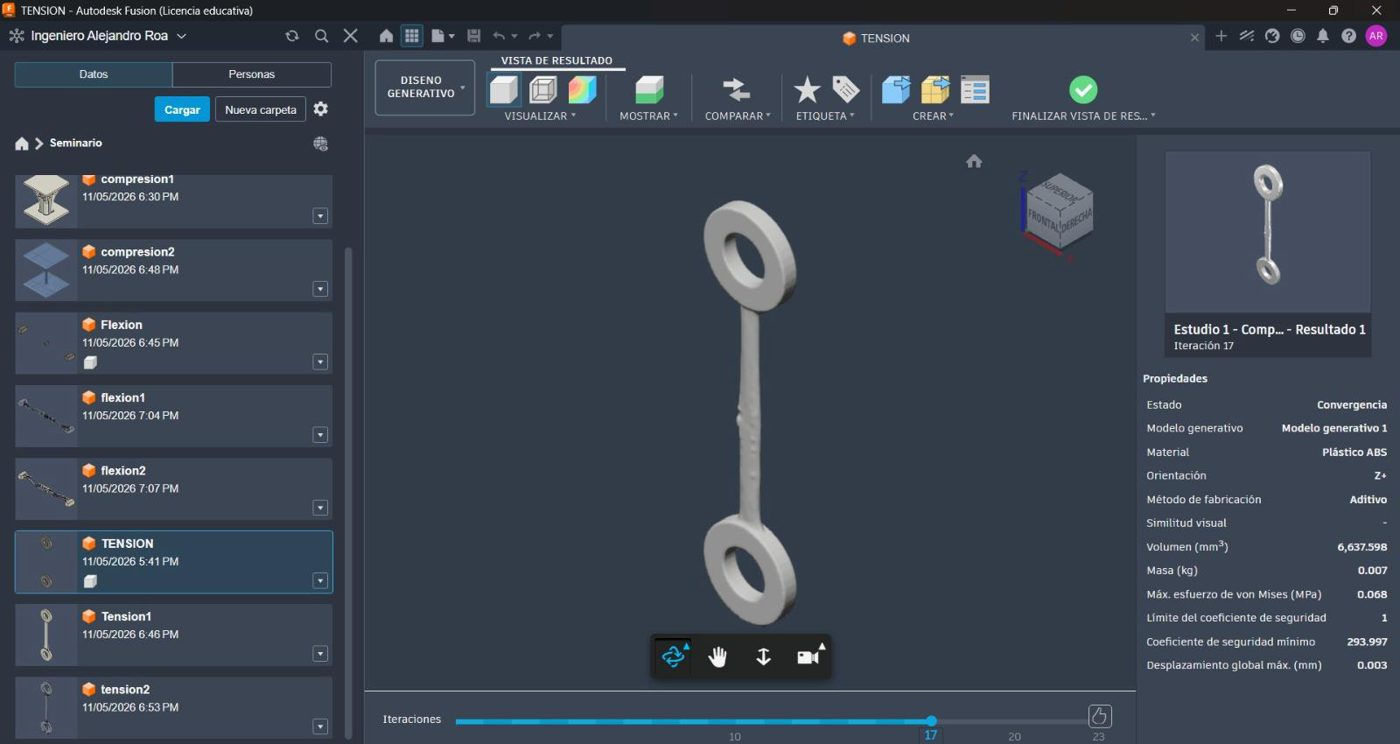
\includegraphics[width=\linewidth,height=0.20\textheight,keepaspectratio]{anexo/p19_1.jpg}\end{subfigure}\hfill
\begin{subfigure}[t]{0.48\textwidth}\centering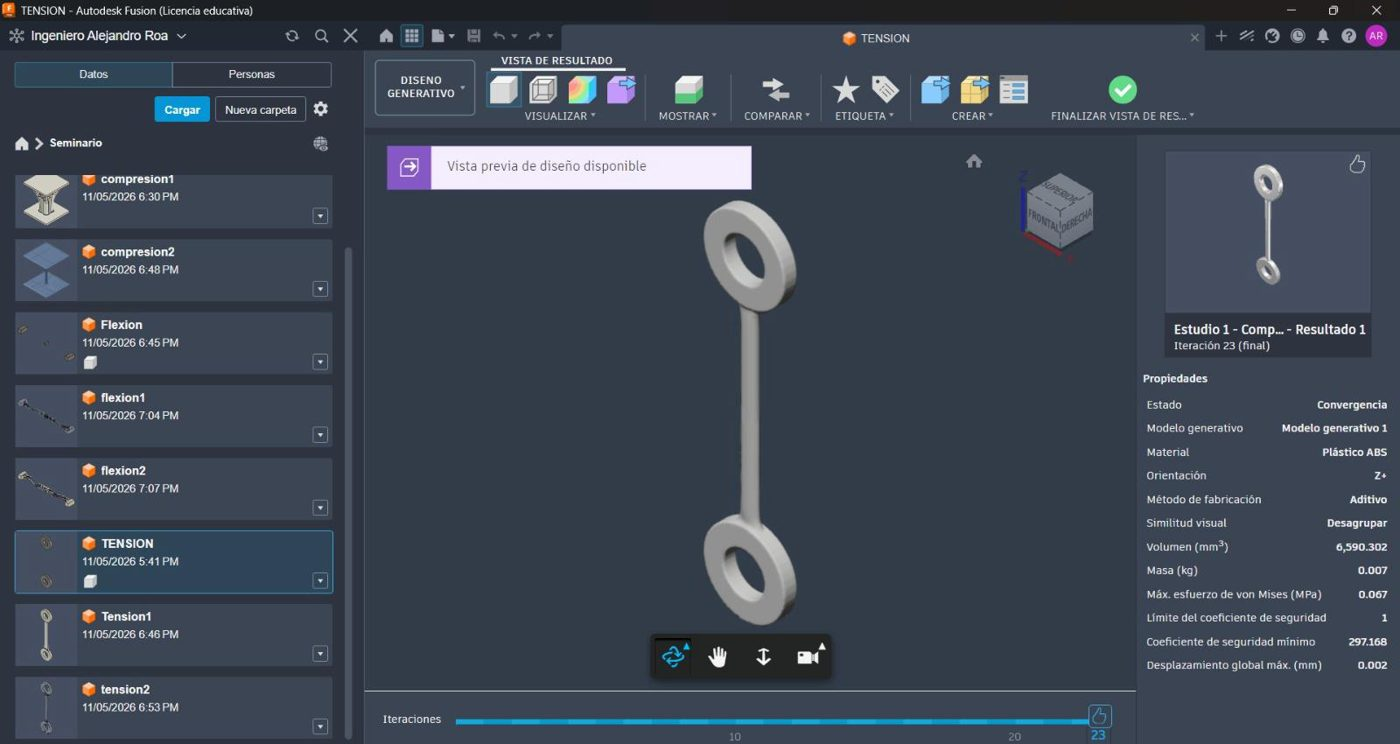
\includegraphics[width=\linewidth,height=0.20\textheight,keepaspectratio]{anexo/p20_0.jpg}\end{subfigure}\par\smallskip
\begin{subfigure}[t]{0.48\textwidth}\centering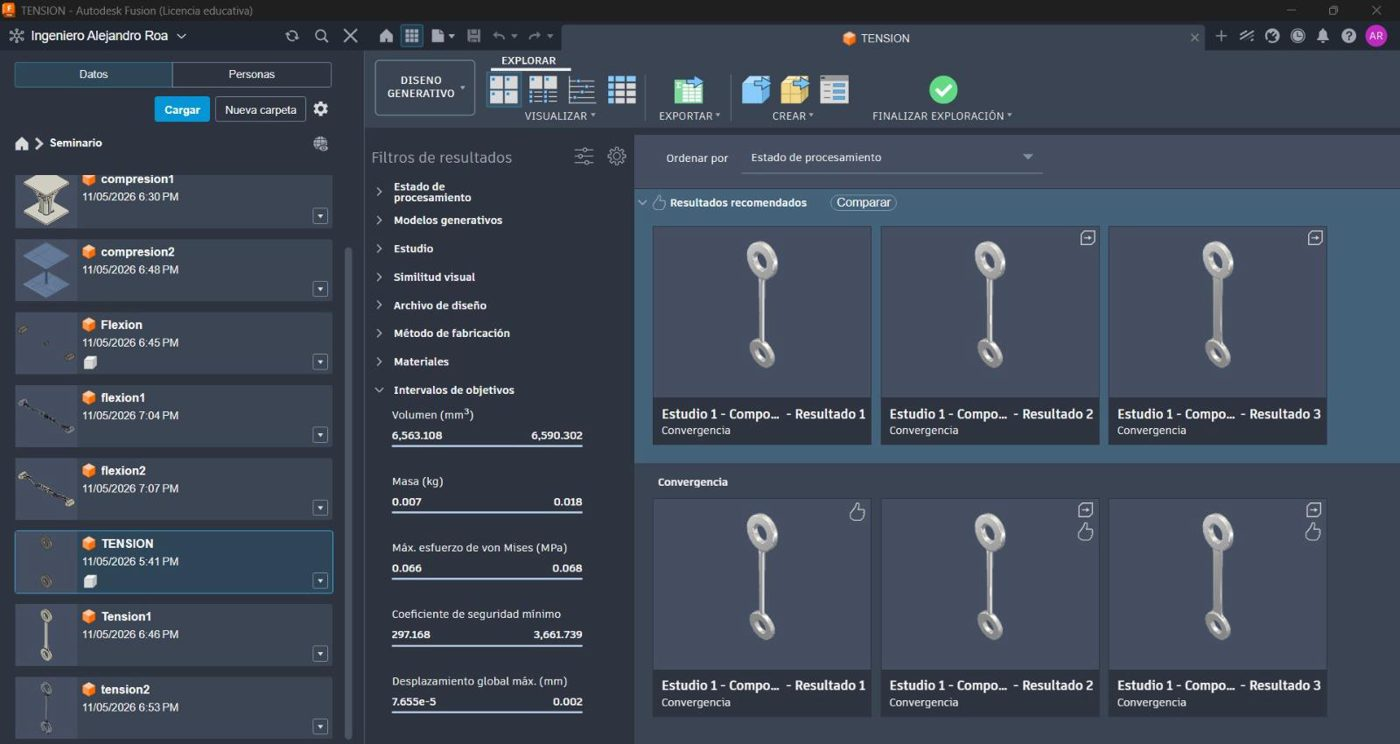
\includegraphics[width=\linewidth,height=0.20\textheight,keepaspectratio]{anexo/p20_1.jpg}\end{subfigure}\hfill
\caption{Diseño generativo de la pieza de tensión en Fusion 360: definición de geometrías y cargas, forma inicial y alternativas generadas.}
\par\footnotesize\textit{Nota.} Elaboración propia. Documento original, páginas 18 a 20.
\end{figure}
\begin{figure}[!htbp]\centering
\begin{subfigure}[t]{0.48\textwidth}\centering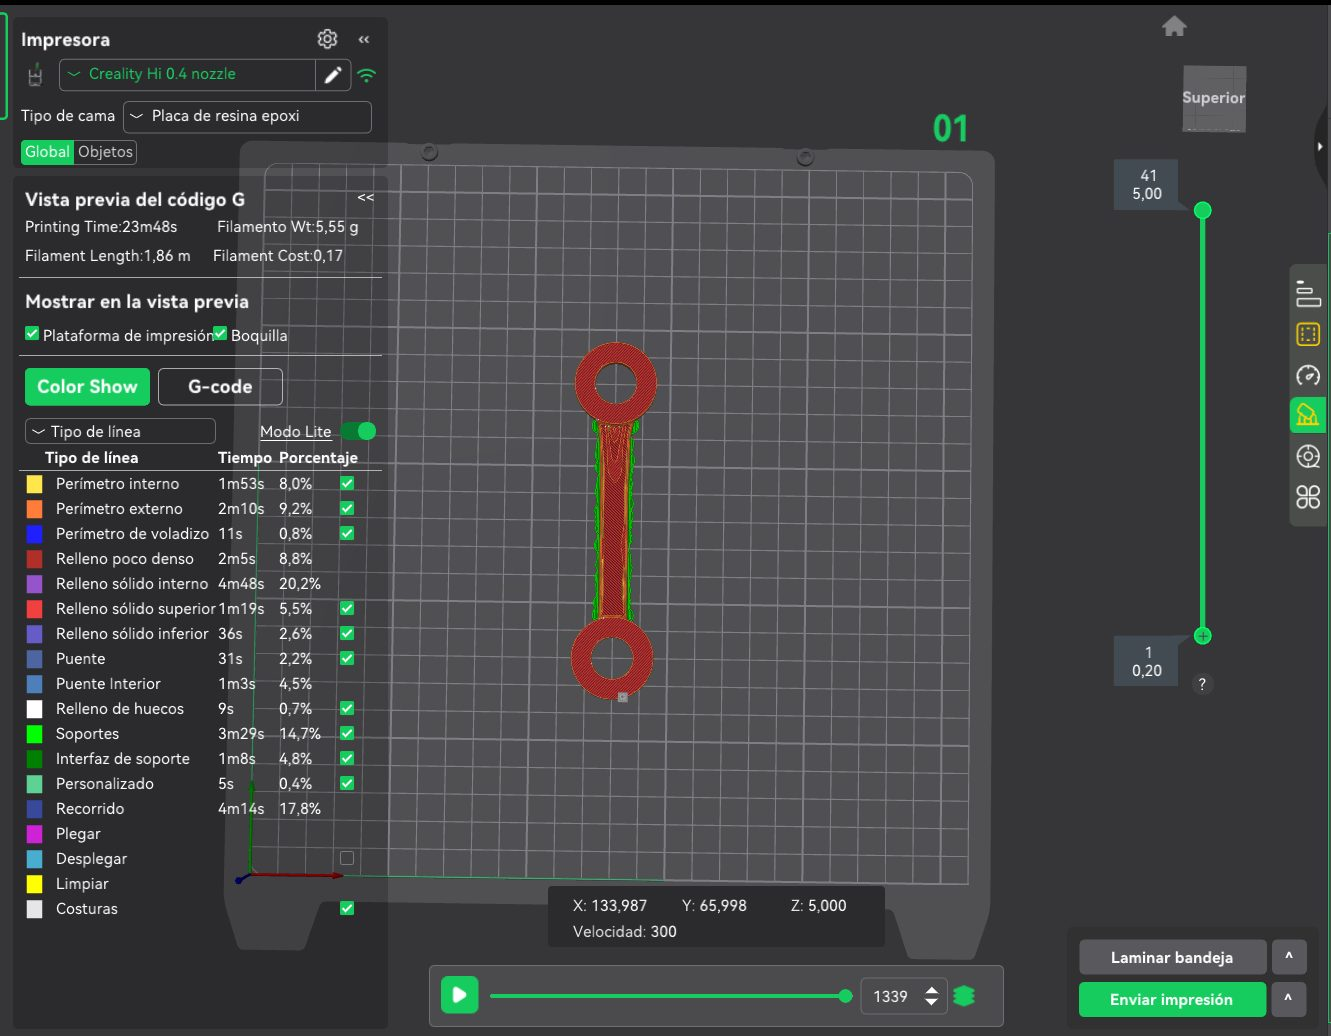
\includegraphics[width=\linewidth,height=0.28\textheight,keepaspectratio]{anexo/p21_0.jpg}\end{subfigure}\hfill
\begin{subfigure}[t]{0.48\textwidth}\centering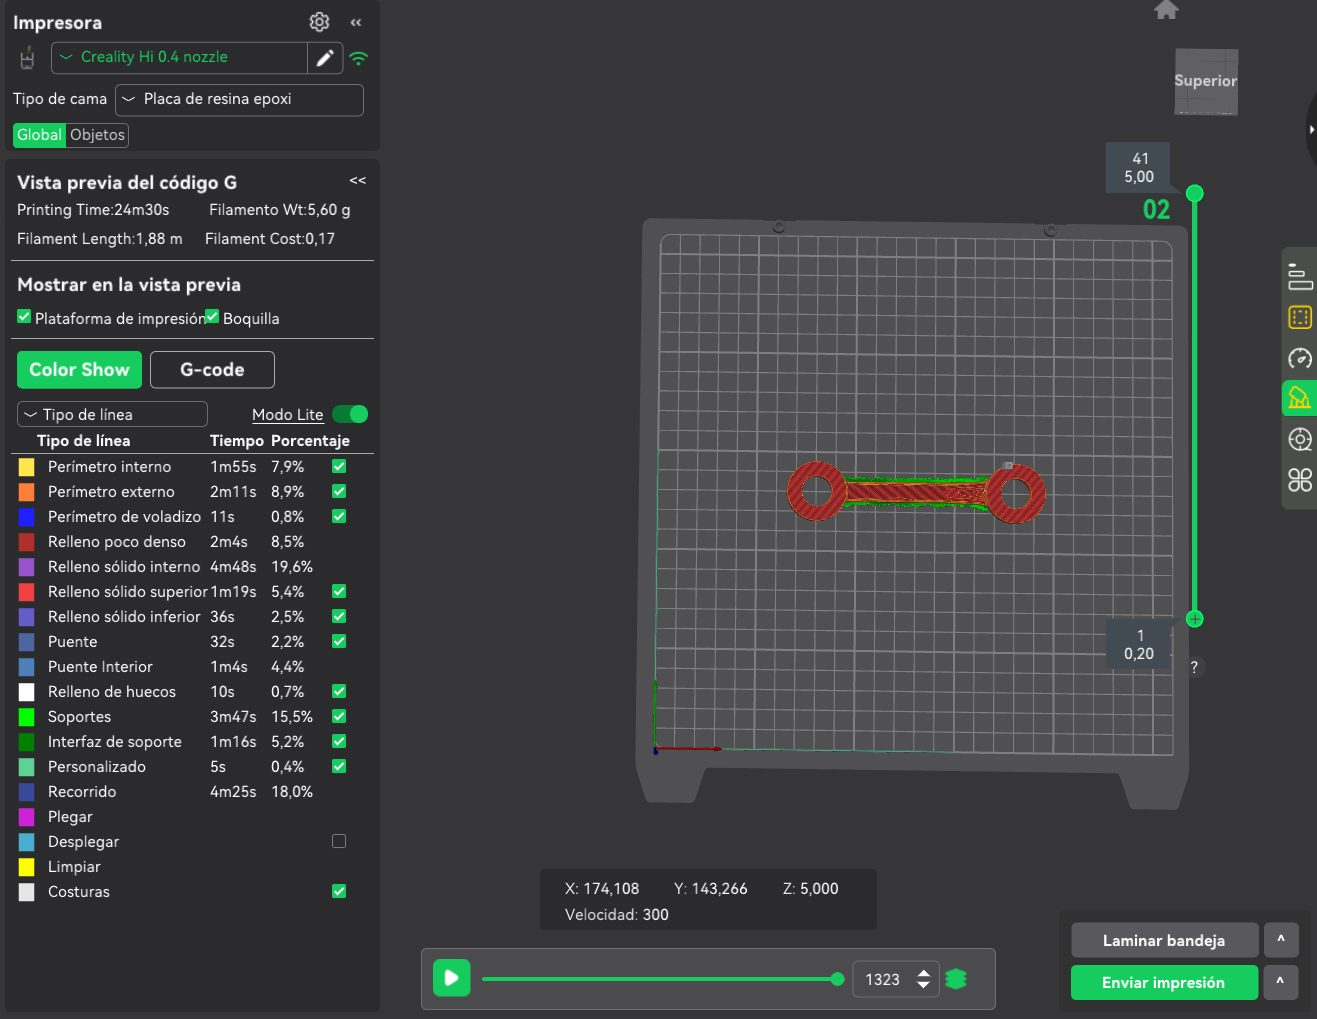
\includegraphics[width=\linewidth,height=0.28\textheight,keepaspectratio]{anexo/p22_0.jpg}\end{subfigure}\par\smallskip
\begin{subfigure}[t]{0.48\textwidth}\centering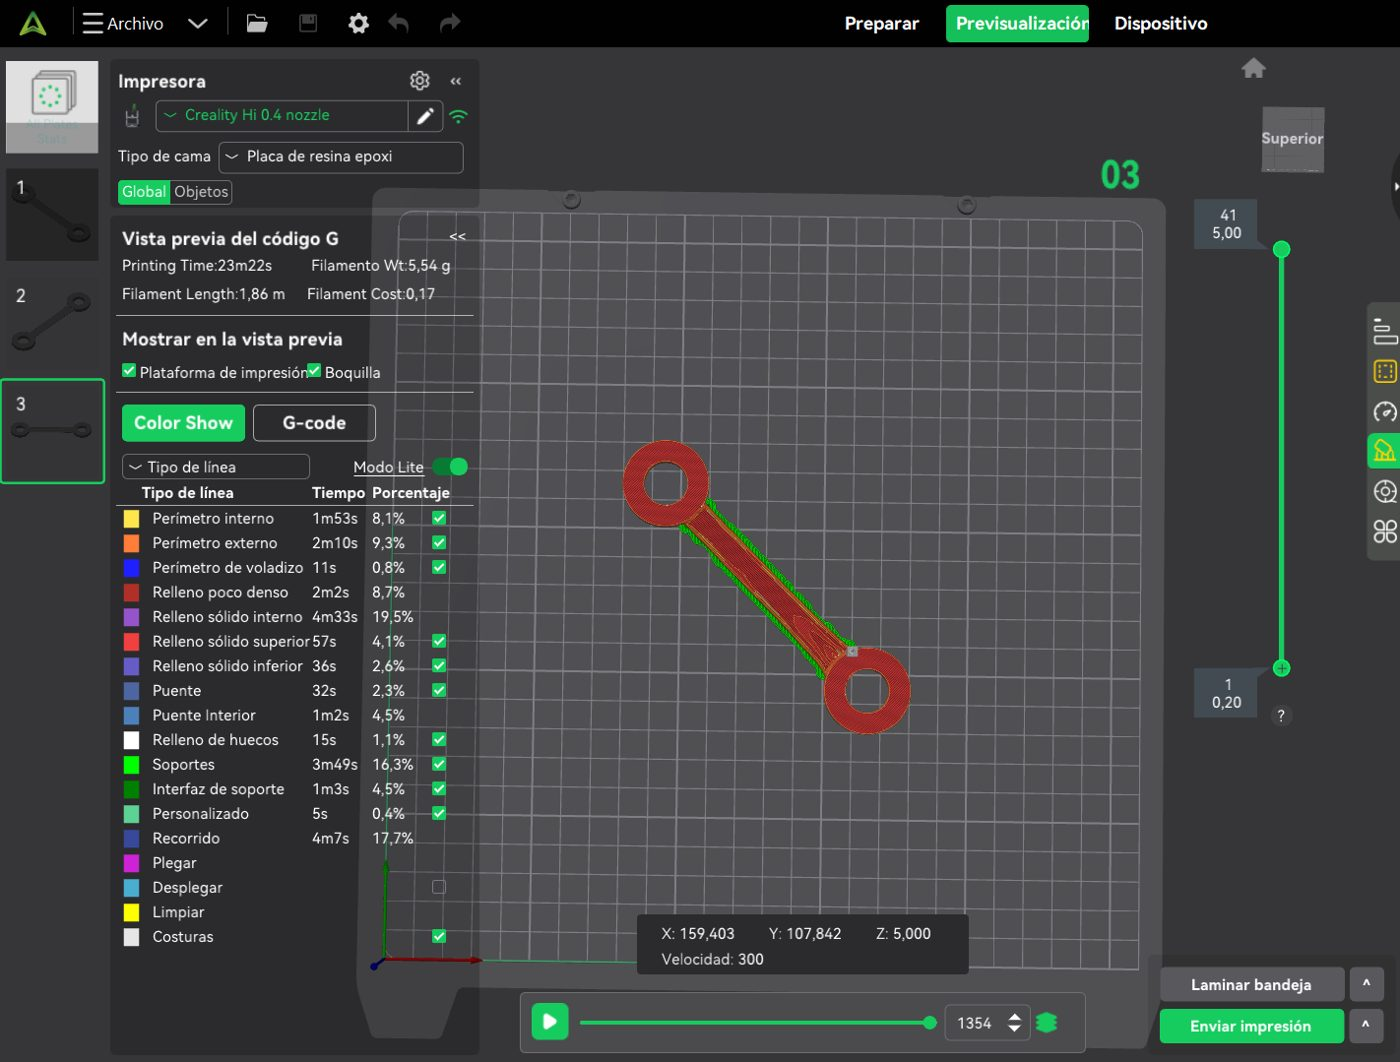
\includegraphics[width=\linewidth,height=0.28\textheight,keepaspectratio]{anexo/p23_0.jpg}\end{subfigure}\hfill
\begin{subfigure}[t]{0.48\textwidth}\centering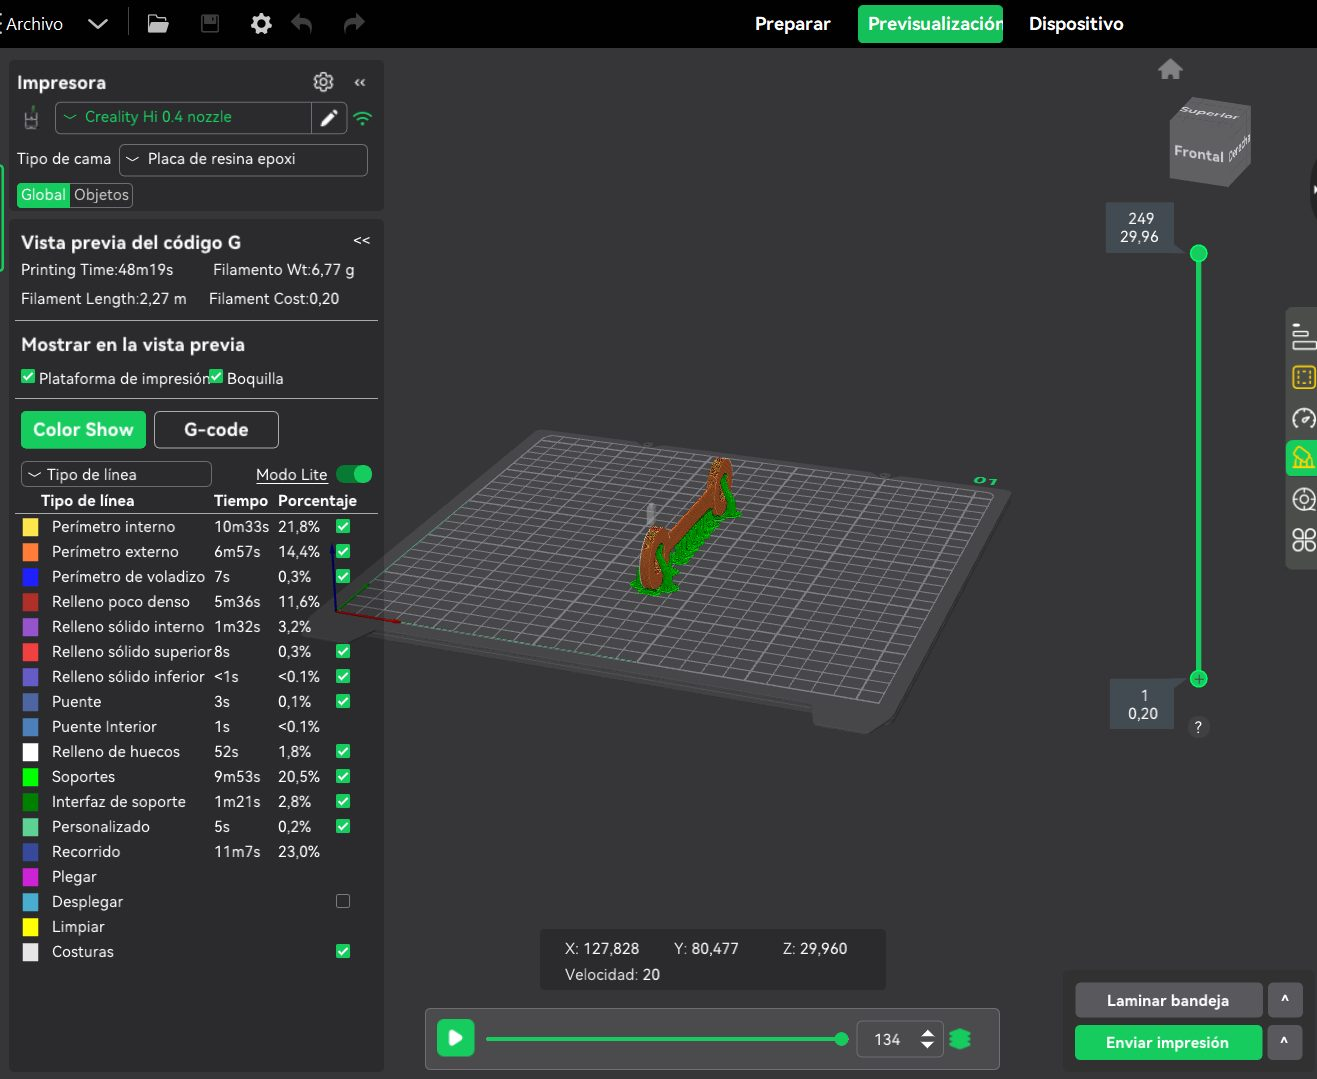
\includegraphics[width=\linewidth,height=0.28\textheight,keepaspectratio]{anexo/p24_0.jpg}\end{subfigure}\par\smallskip
\caption{Vistas de laminado en Creality Print con distintas orientaciones (1 de 3).}
\par\footnotesize\textit{Nota.} Elaboración propia. Documento original, páginas 21 a 24.
\end{figure}
\begin{figure}[!htbp]\centering
\begin{subfigure}[t]{0.48\textwidth}\centering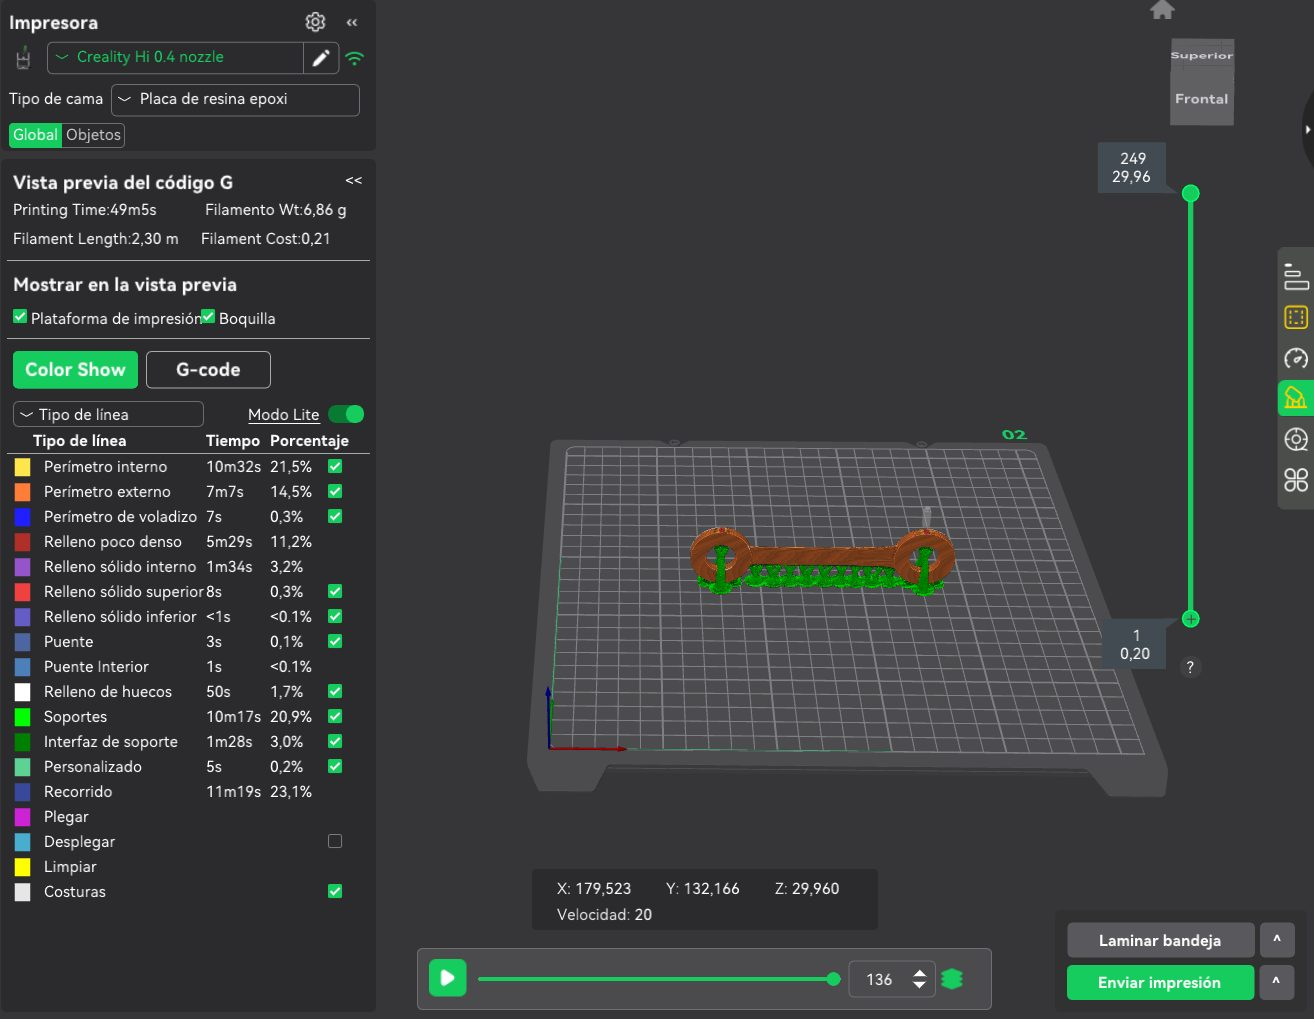
\includegraphics[width=\linewidth,height=0.28\textheight,keepaspectratio]{anexo/p25_0.jpg}\end{subfigure}\hfill
\begin{subfigure}[t]{0.48\textwidth}\centering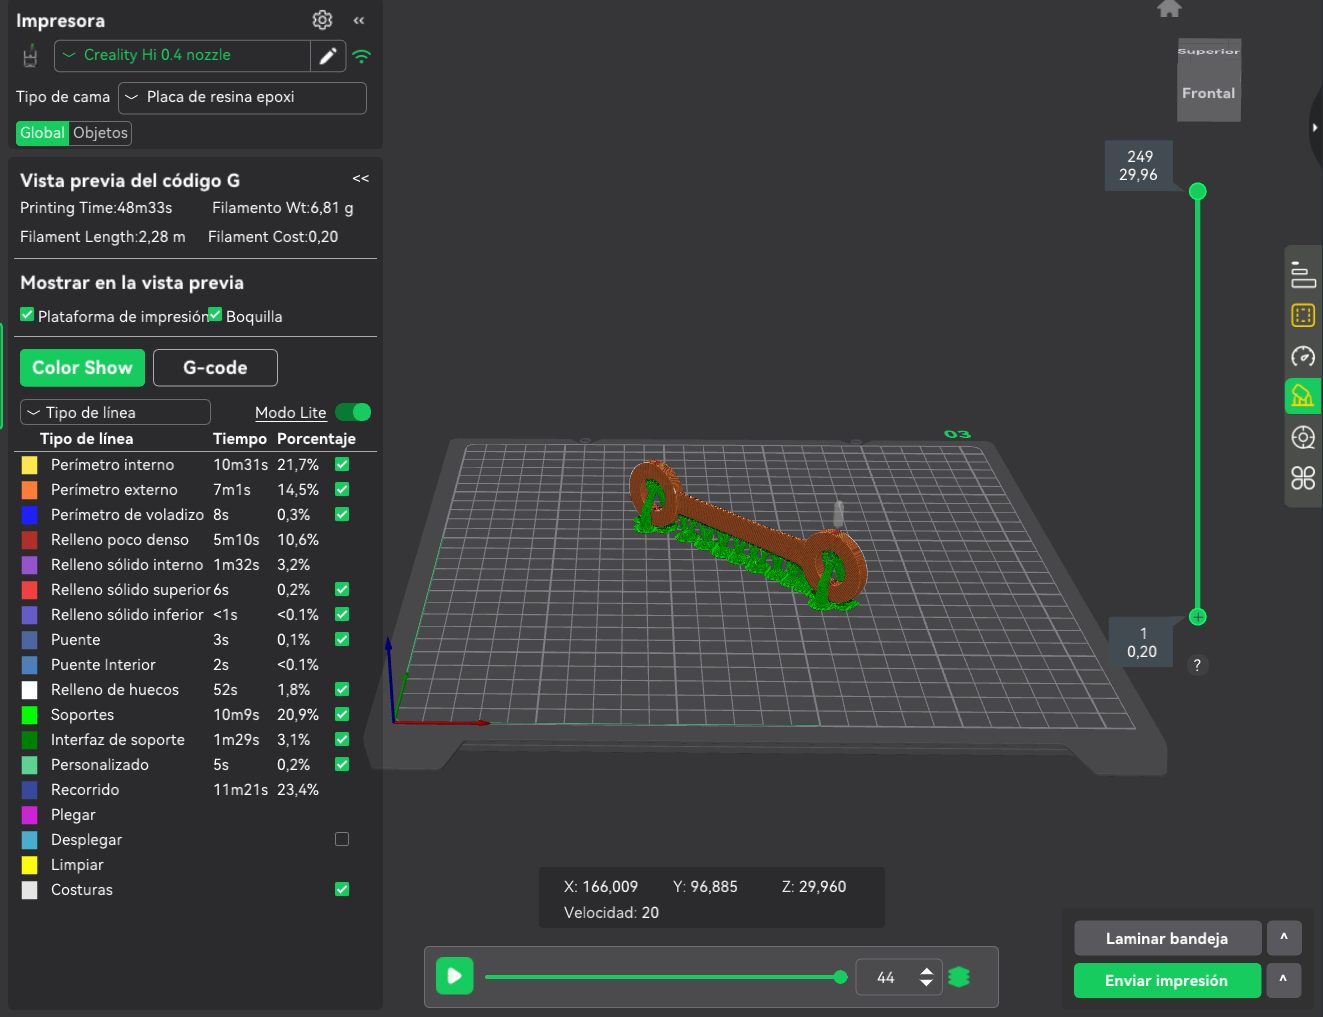
\includegraphics[width=\linewidth,height=0.28\textheight,keepaspectratio]{anexo/p26_0.jpg}\end{subfigure}\par\smallskip
\begin{subfigure}[t]{0.48\textwidth}\centering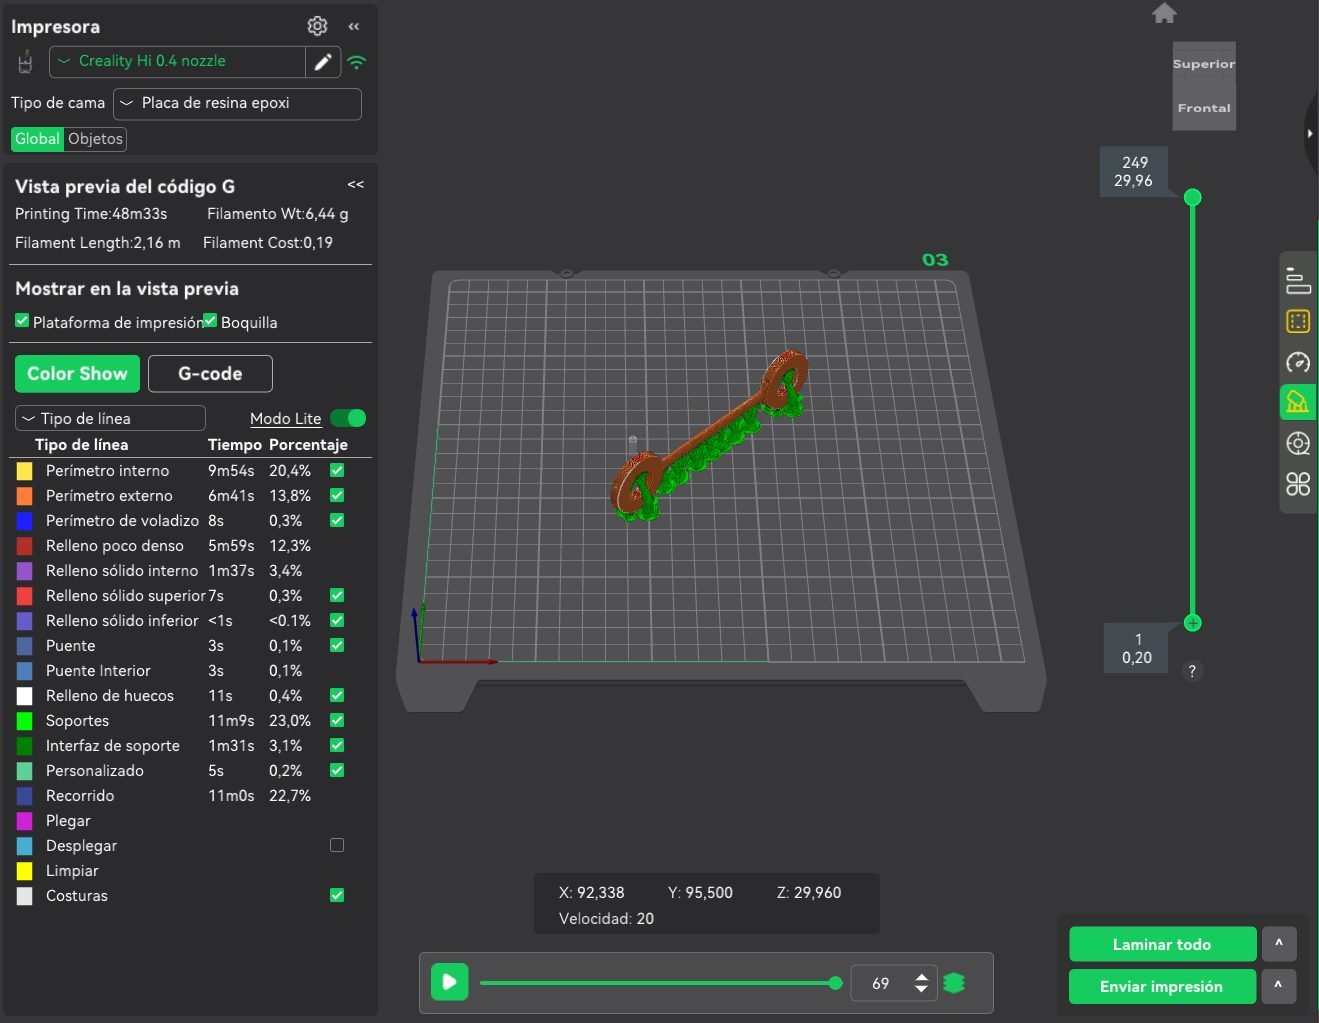
\includegraphics[width=\linewidth,height=0.28\textheight,keepaspectratio]{anexo/p27_0.jpg}\end{subfigure}\hfill
\begin{subfigure}[t]{0.48\textwidth}\centering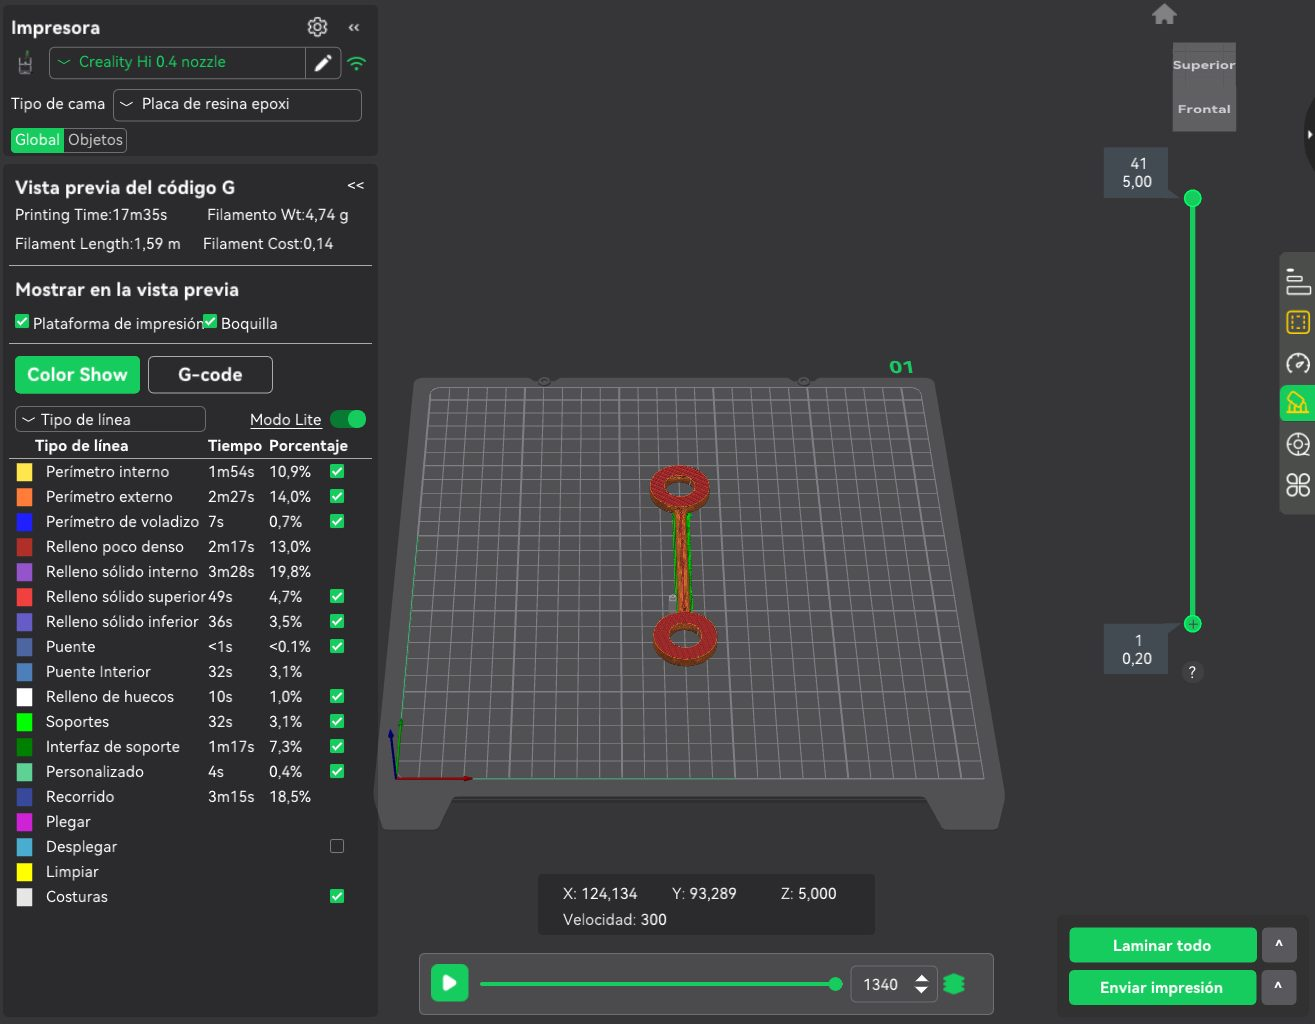
\includegraphics[width=\linewidth,height=0.28\textheight,keepaspectratio]{anexo/p28_0.jpg}\end{subfigure}\par\smallskip
\caption{Vistas de laminado en Creality Print con distintas orientaciones (2 de 3).}
\par\footnotesize\textit{Nota.} Elaboración propia. Documento original, páginas 25 a 28.
\end{figure}
\begin{figure}[!htbp]\centering
\begin{subfigure}[t]{0.48\textwidth}\centering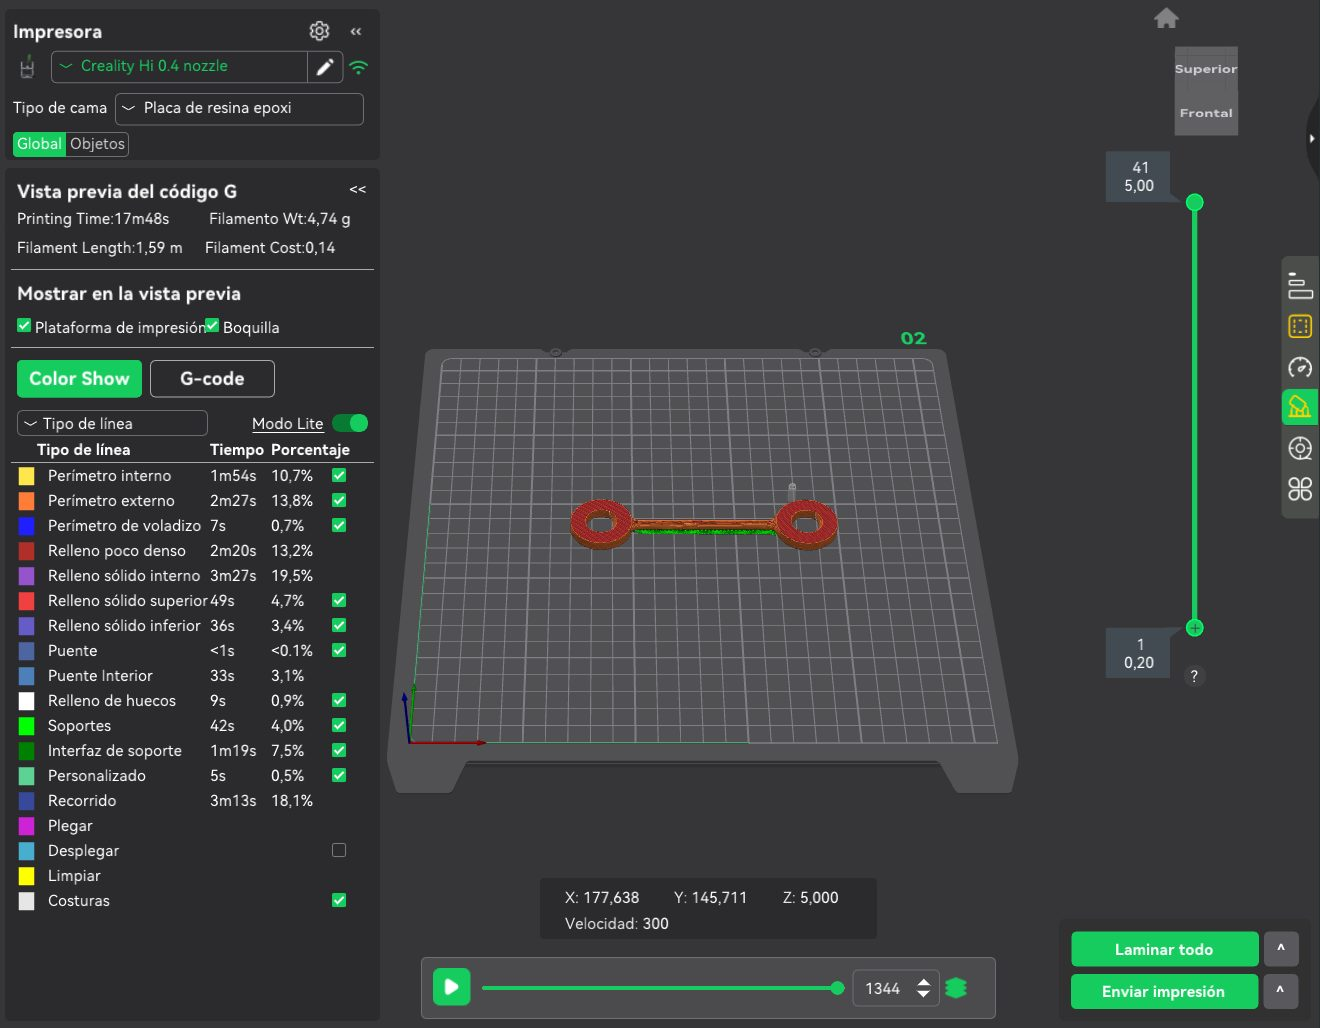
\includegraphics[width=\linewidth,height=0.28\textheight,keepaspectratio]{anexo/p29_0.jpg}\end{subfigure}\hfill
\begin{subfigure}[t]{0.48\textwidth}\centering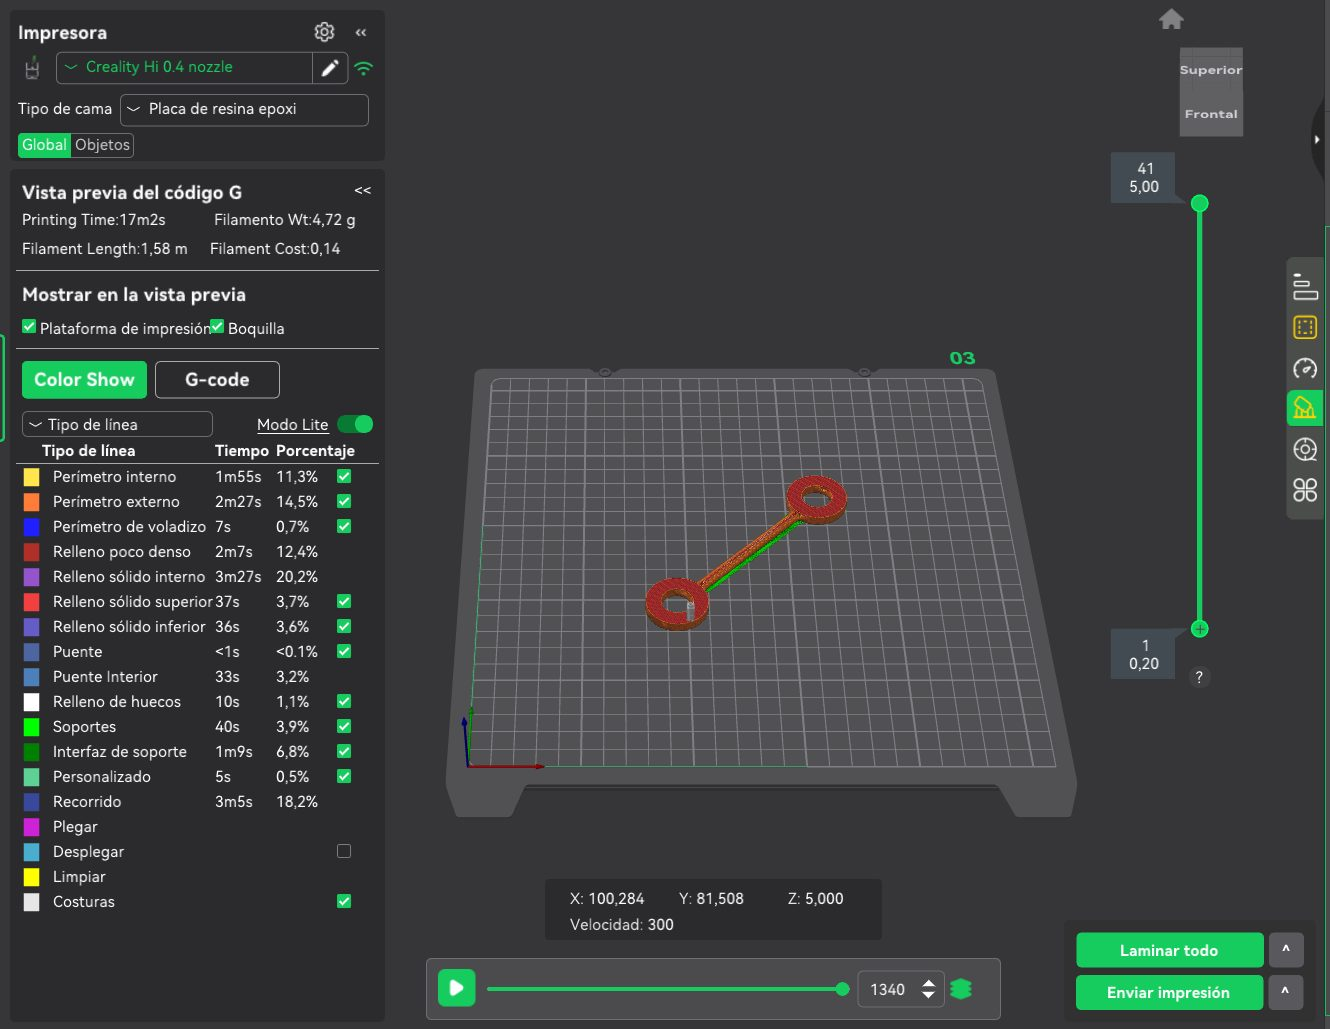
\includegraphics[width=\linewidth,height=0.28\textheight,keepaspectratio]{anexo/p30_0.jpg}\end{subfigure}\par\smallskip
\begin{subfigure}[t]{0.48\textwidth}\centering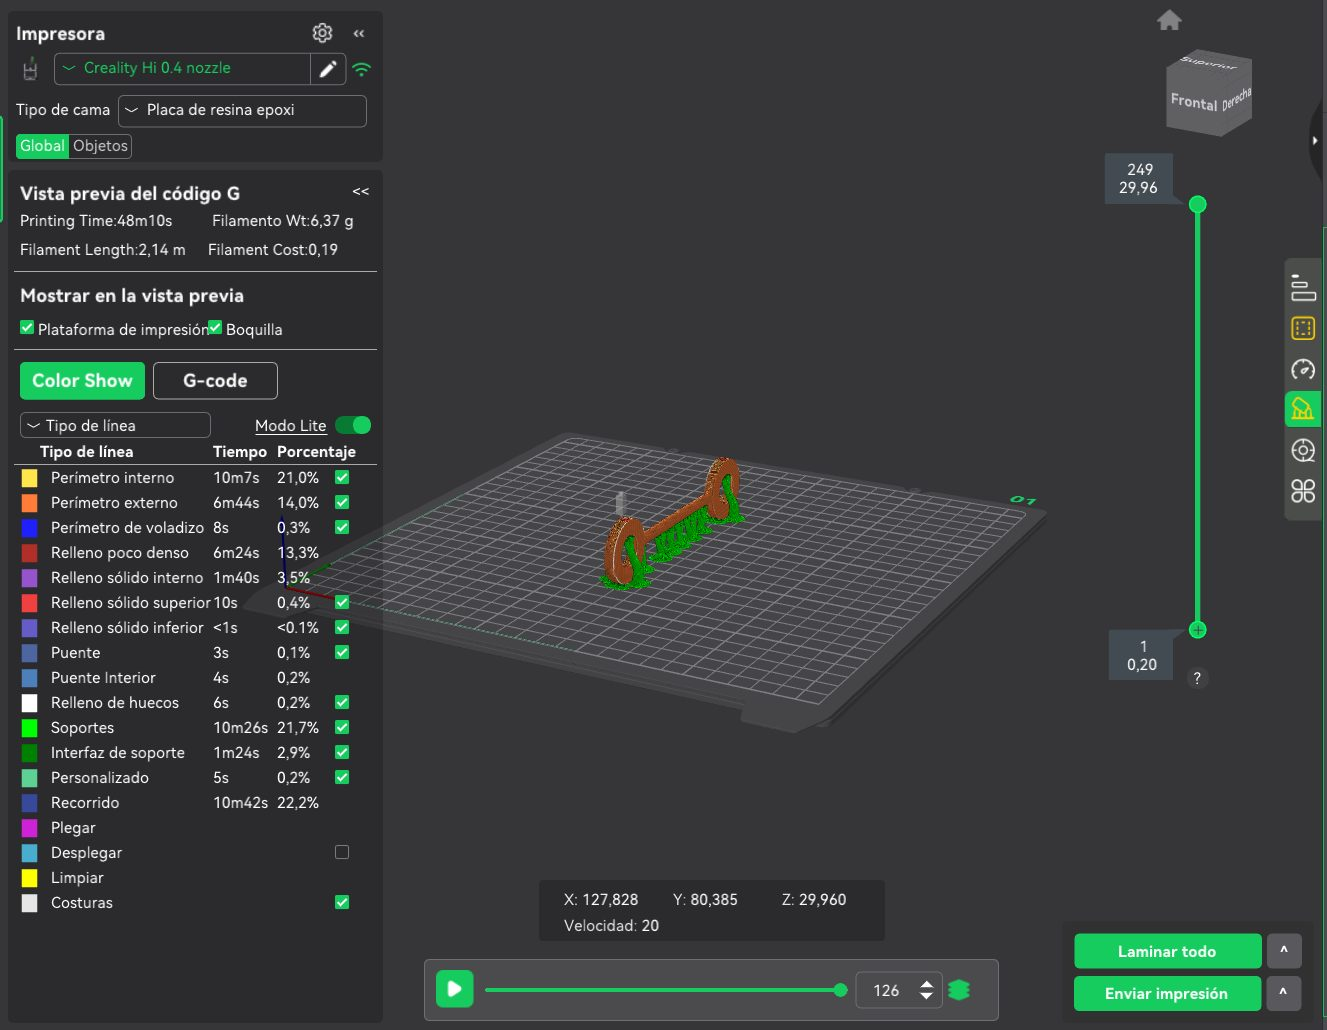
\includegraphics[width=\linewidth,height=0.28\textheight,keepaspectratio]{anexo/p31_0.jpg}\end{subfigure}\hfill
\begin{subfigure}[t]{0.48\textwidth}\centering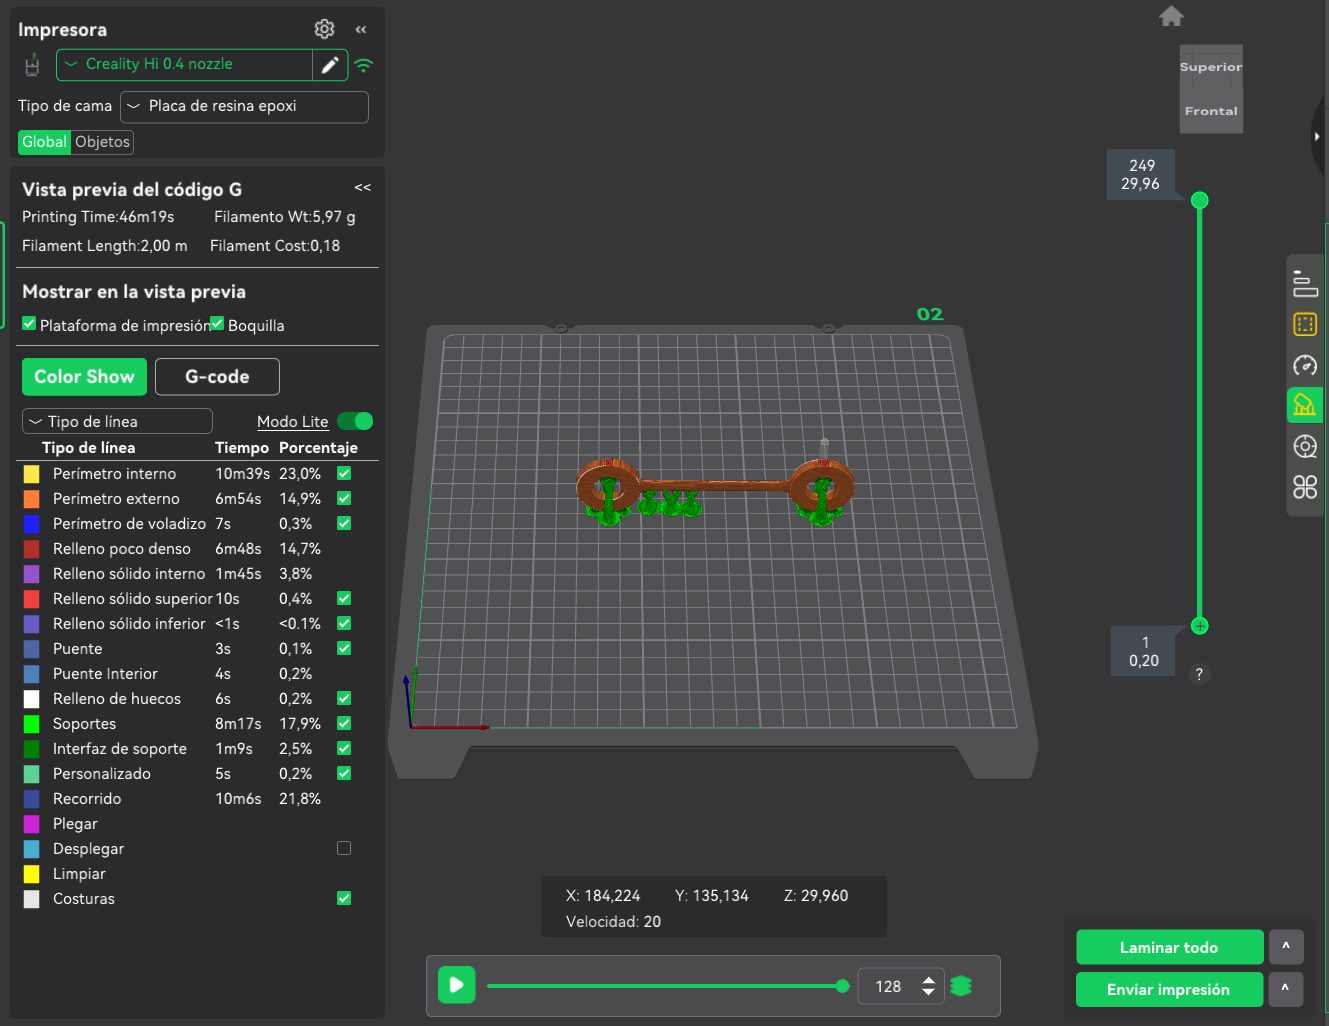
\includegraphics[width=\linewidth,height=0.28\textheight,keepaspectratio]{anexo/p32_0.jpg}\end{subfigure}\par\smallskip
\caption{Vistas de laminado en Creality Print con distintas orientaciones (3 de 3).}
\par\footnotesize\textit{Nota.} Elaboración propia. Documento original, páginas 29 a 32.
\end{figure}
\begin{figure}[!htbp]\centering
\begin{subfigure}[t]{0.48\textwidth}\centering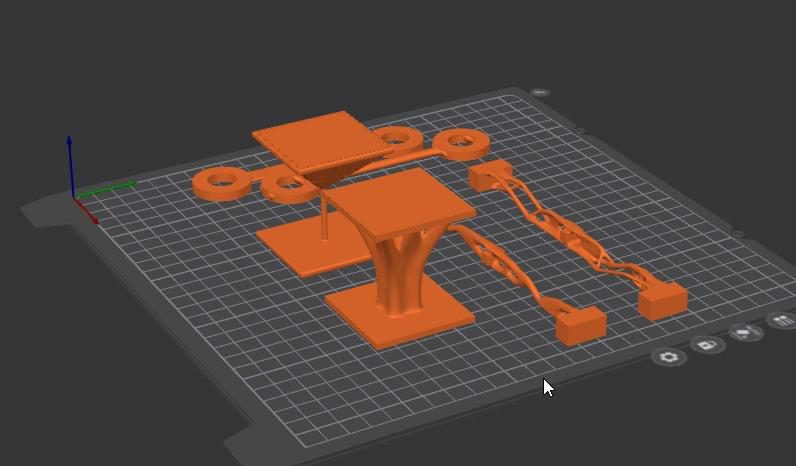
\includegraphics[width=\linewidth,height=0.28\textheight,keepaspectratio]{anexo/p33_0.jpg}\end{subfigure}\hfill
\begin{subfigure}[t]{0.48\textwidth}\centering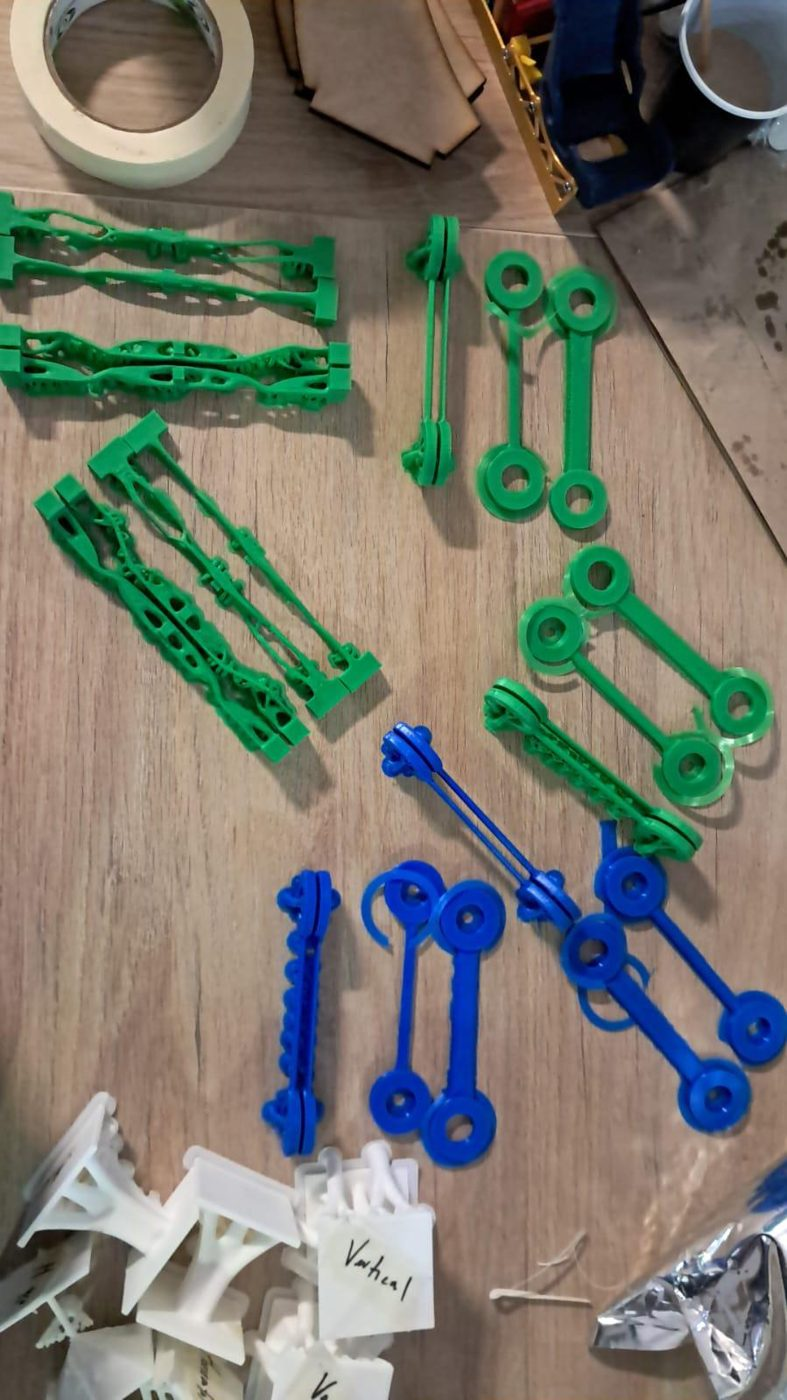
\includegraphics[width=\linewidth,height=0.28\textheight,keepaspectratio]{anexo/p33_1.jpg}\end{subfigure}\par\smallskip
\begin{subfigure}[t]{0.48\textwidth}\centering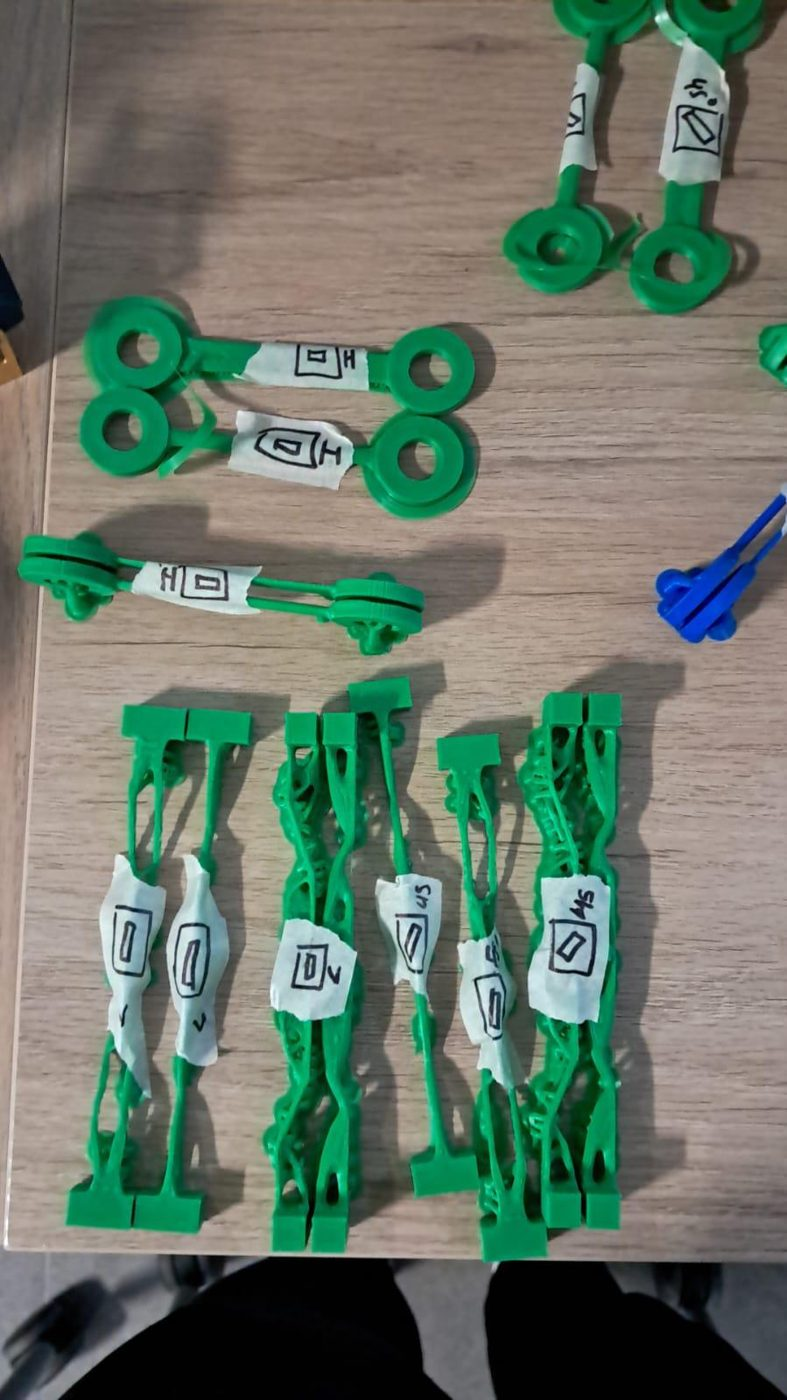
\includegraphics[width=\linewidth,height=0.28\textheight,keepaspectratio]{anexo/p34_0.jpg}\end{subfigure}\hfill
\begin{subfigure}[t]{0.48\textwidth}\centering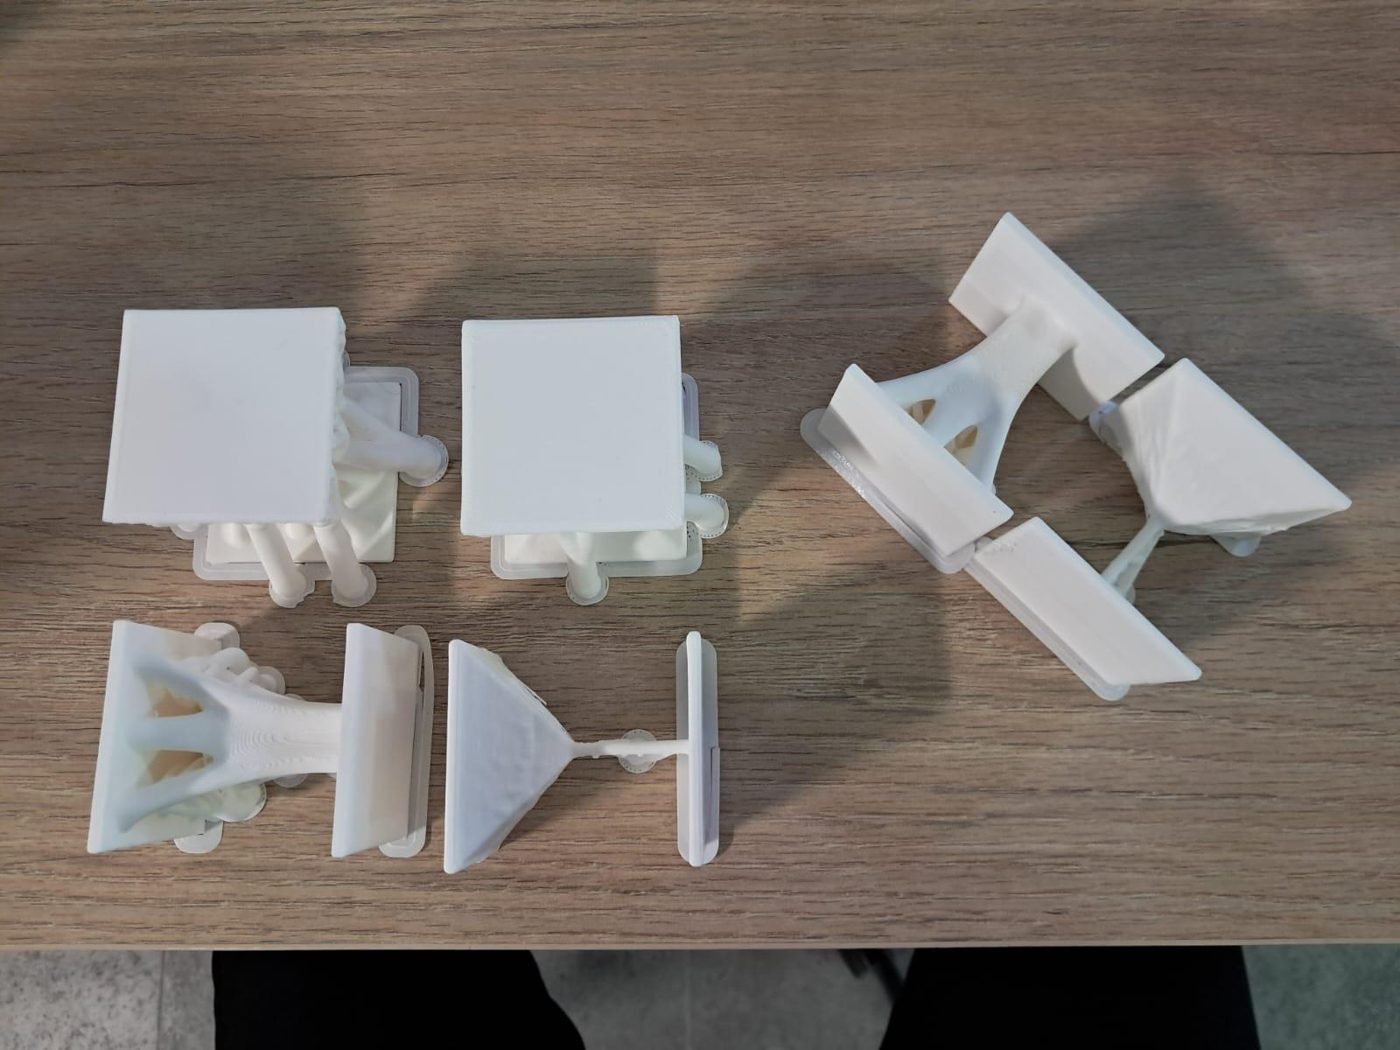
\includegraphics[width=\linewidth,height=0.28\textheight,keepaspectratio]{anexo/p34_1.jpg}\end{subfigure}\par\smallskip
\caption{Distribución de las piezas en la cama de impresión y piezas fabricadas.}
\par\footnotesize\textit{Nota.} Elaboración propia. Documento original, páginas 33 y 34.
\end{figure}
\endgroup

\end{document}
